%%%%%%%%%%%%%%%%%%%%%%%%%%%%%%%%%%%%%%%%%%  不使用 authblk 包制作标题  %%%%%%%%%%%%%%%%%%%%%%%%%%%%%%%%%%%%%%%%%%%%%%
%-------------------------------PPT Title-------------------------------------
\title{10-第一原理分子动力学概要}
%-----------------------------------------------------------------------------
%----------------------------Author & Date------------------------------------

%\author[\textrm{Jun\_Jiang}]{姜\;\;骏\inst{}} %[]{} (optional, use only with lots of authors)
%% - Give the names in the same order as the appear in the paper.
%% - Use the \inst{?} command only if the authors have different
%%   affiliation.
%\institute[BCC]{\inst{}%
\institute[Gain~Strong]{\inst{}%
%\vskip -20pt 北京市计算中心}
\vskip -20pt {\large 格致斯创~科技}}
\date[\today] % (optional, should be abbreviation of conference name)
{%	{\fontsize{6.2pt}{4.2pt}\selectfont{\textcolor{blue}{E-mail:~}\url{jiangjun@bcc.ac.cn}}}
\vskip 45 pt {\fontsize{8.2pt}{6.2pt}\selectfont{%清华大学\;\;物理系% 报告地点
	\vskip 5 pt \textrm{2023.04.08}}}
}

%% - Either use conference name or its abbreviation
%% - Not really information to the audience, more for people (including
%%   yourself) who are reading the slides onlin%%   yourself) who are reading the slides onlin%%   yourself) who are reading the slides onlineee
%%%%%%%%%%%%%%%%%%%%%%%%%%%%%%%%%%%%%%%%%%%%%%%%%%%%%%%%%%%%%%%%%%%%%%%%%%%%%%%%%%%%%%%%%%%%%%%%%%%%%%%%%%%%%%%%%%%%%

\subject{}
% This is only inserted into the PDF information catalog. Can be left
% out.
%\maketitle
\frame
{
%	\frametitle{\fontsize{9.5pt}{5.2pt}\selectfont{\textcolor{orange}{“高通量并发式材料计算算法与软件”年度检查}}}
\titlepage
}
%-----------------------------------------------------------------------------

%------------------------------------------------------------------------------列出全文 outline ---------------------------------------------------------------------------------
%\section*{}
%\frame[allowframebreaks]
%{
%  \frametitle{Outline}
%%  \frametitle{\textcolor{mycolor}{\secname}}
%  \tableofcontents%[current,currentsection,currentsubsection]
%}
%%在每个section之前列出全部Outline
%%类似的在每个subsection之前列出全部Outline是\AtBeginSubsection[]
%\AtBeginSection[]
%{
%  \frame<handout:0>%[allowframebreaks]
%  {
%    \frametitle{Outline}
%%全部Outline中,本部分加亮
%    \tableofcontents[current,currentsection]
%  }
%}

%-----------------------------------------------PPT main Body------------------------------------------------------------------------------------
\small
%\section{\rm{VASP~}软件中\rm{PAW~}计算的实现}
%\frame
%
%	\frametitle{\textrm{VASP}计算的特色}
%	相比于与普通的第一原理计算软件,\textrm{VASP}很好地平衡了计算效率和精度的问题,总的来说,\textrm{VASP}主要通过这几个特色保证了计算的高效能
%	\begin{itemize}
%	     \item 迭代与优化算法的多样性\\
%		     本质上电荷密度迭代 \textrm{\&\&} 体系总能量优化是相同的优化问题,采用了类似的算法\upcite{CMS6-15_1996,PRB54-11169_1996}:\\
%			\textcolor{blue}{\textrm{Pseudo-Newton、Conjugate-Gradient、Broyden~mix、damping-factor、RMM-DIIS}}
%	     \item 尽可能采用局域基(原子轨道基)函数:~\\
%		     \textcolor{blue}{\textrm{LREAL}}=\textcolor{red}{\textrm{.TRUE.}}\\
%			优化的投影函数也尽可能在实空间表示
%	     \item \textrm{PAW}原子数据集:\textcolor{blue}{优异的赝势}\upcite{PRB59-1758_1999}
%	\end{itemize}
%}
\subsection{\textrm{VASP}中的电荷密度混合与矩阵迭代对角化}
\frame
{
	\frametitle{不动点问题}
	求解方程
	\begin{displaymath}
		f(\mathbf{x})=\mathbf{x}
	\end{displaymath}
	$\mathbf{x}$是函数$f(\mathbf{x})$的\textcolor{red}{不动点}\textrm{Fixed Point}
	
	对这类问题的求解,可以利用迭代关系
	\begin{displaymath}
		\mathbf{x}_{i+1}=f(\mathbf{x}_i)\qquad (i=1,2,3,\cdots)
	\end{displaymath}
	这称为\textcolor{blue}{不动点迭代法}

	{\fontsize{6.2pt}{4.2pt}\selectfont{例如求解方程
	\begin{displaymath}
%		\begin{aligned}
			\lg(10+x)~=~x%\\
			\Longrightarrow	\textcolor{blue}{x\approx 1.04309063}
%		\end{aligned}
		\end{displaymath}}}
\begin{minipage}[b]{0.35\textwidth}
		{\fontsize{3.2pt}{1.2pt}\selectfont{
	\begin{displaymath}
	\vspace{-0.11in}
		\begin{aligned}
			x_0&=1 %~\Longrightarrow 
			\\\lg(10+1)&=1.041392685\\
x_1 &=1.041392685 %~\Longrightarrow 
\\\lg(10+1.041392685)&=1.0430238558\\
x_2 &=1.043023856 %~\Longrightarrow 
\\\lg(10+1.043023856)&=1.0430880104\\
x_3 &=1.043088010 %~\Longrightarrow 
\\\lg(10+1.043088010)&=1.0443090533\\
x_4 &=1.043090533 %~\Longrightarrow 
\\\lg(10+1.043090533)&=1.04430906326\\
x_4 &=1.0430906326 %~\Longrightarrow 
\\\lg(10+1.0430906326)&=1.04430906365\\
x_5 &=1.0430906365 %~\Longrightarrow 
\\\lg(10+1.0430906365)&=1.04430906366\\
x_6 &=1.0430906366 %~\Longrightarrow 
\\\lg(10+1.0430906366)&=1.04430906366
		\end{aligned}
	\end{displaymath}}}
\end{minipage}
\hfill
\begin{minipage}[b]{0.62\textwidth}
\begin{figure}[h!]
	\vspace{-0.21in}
\centering
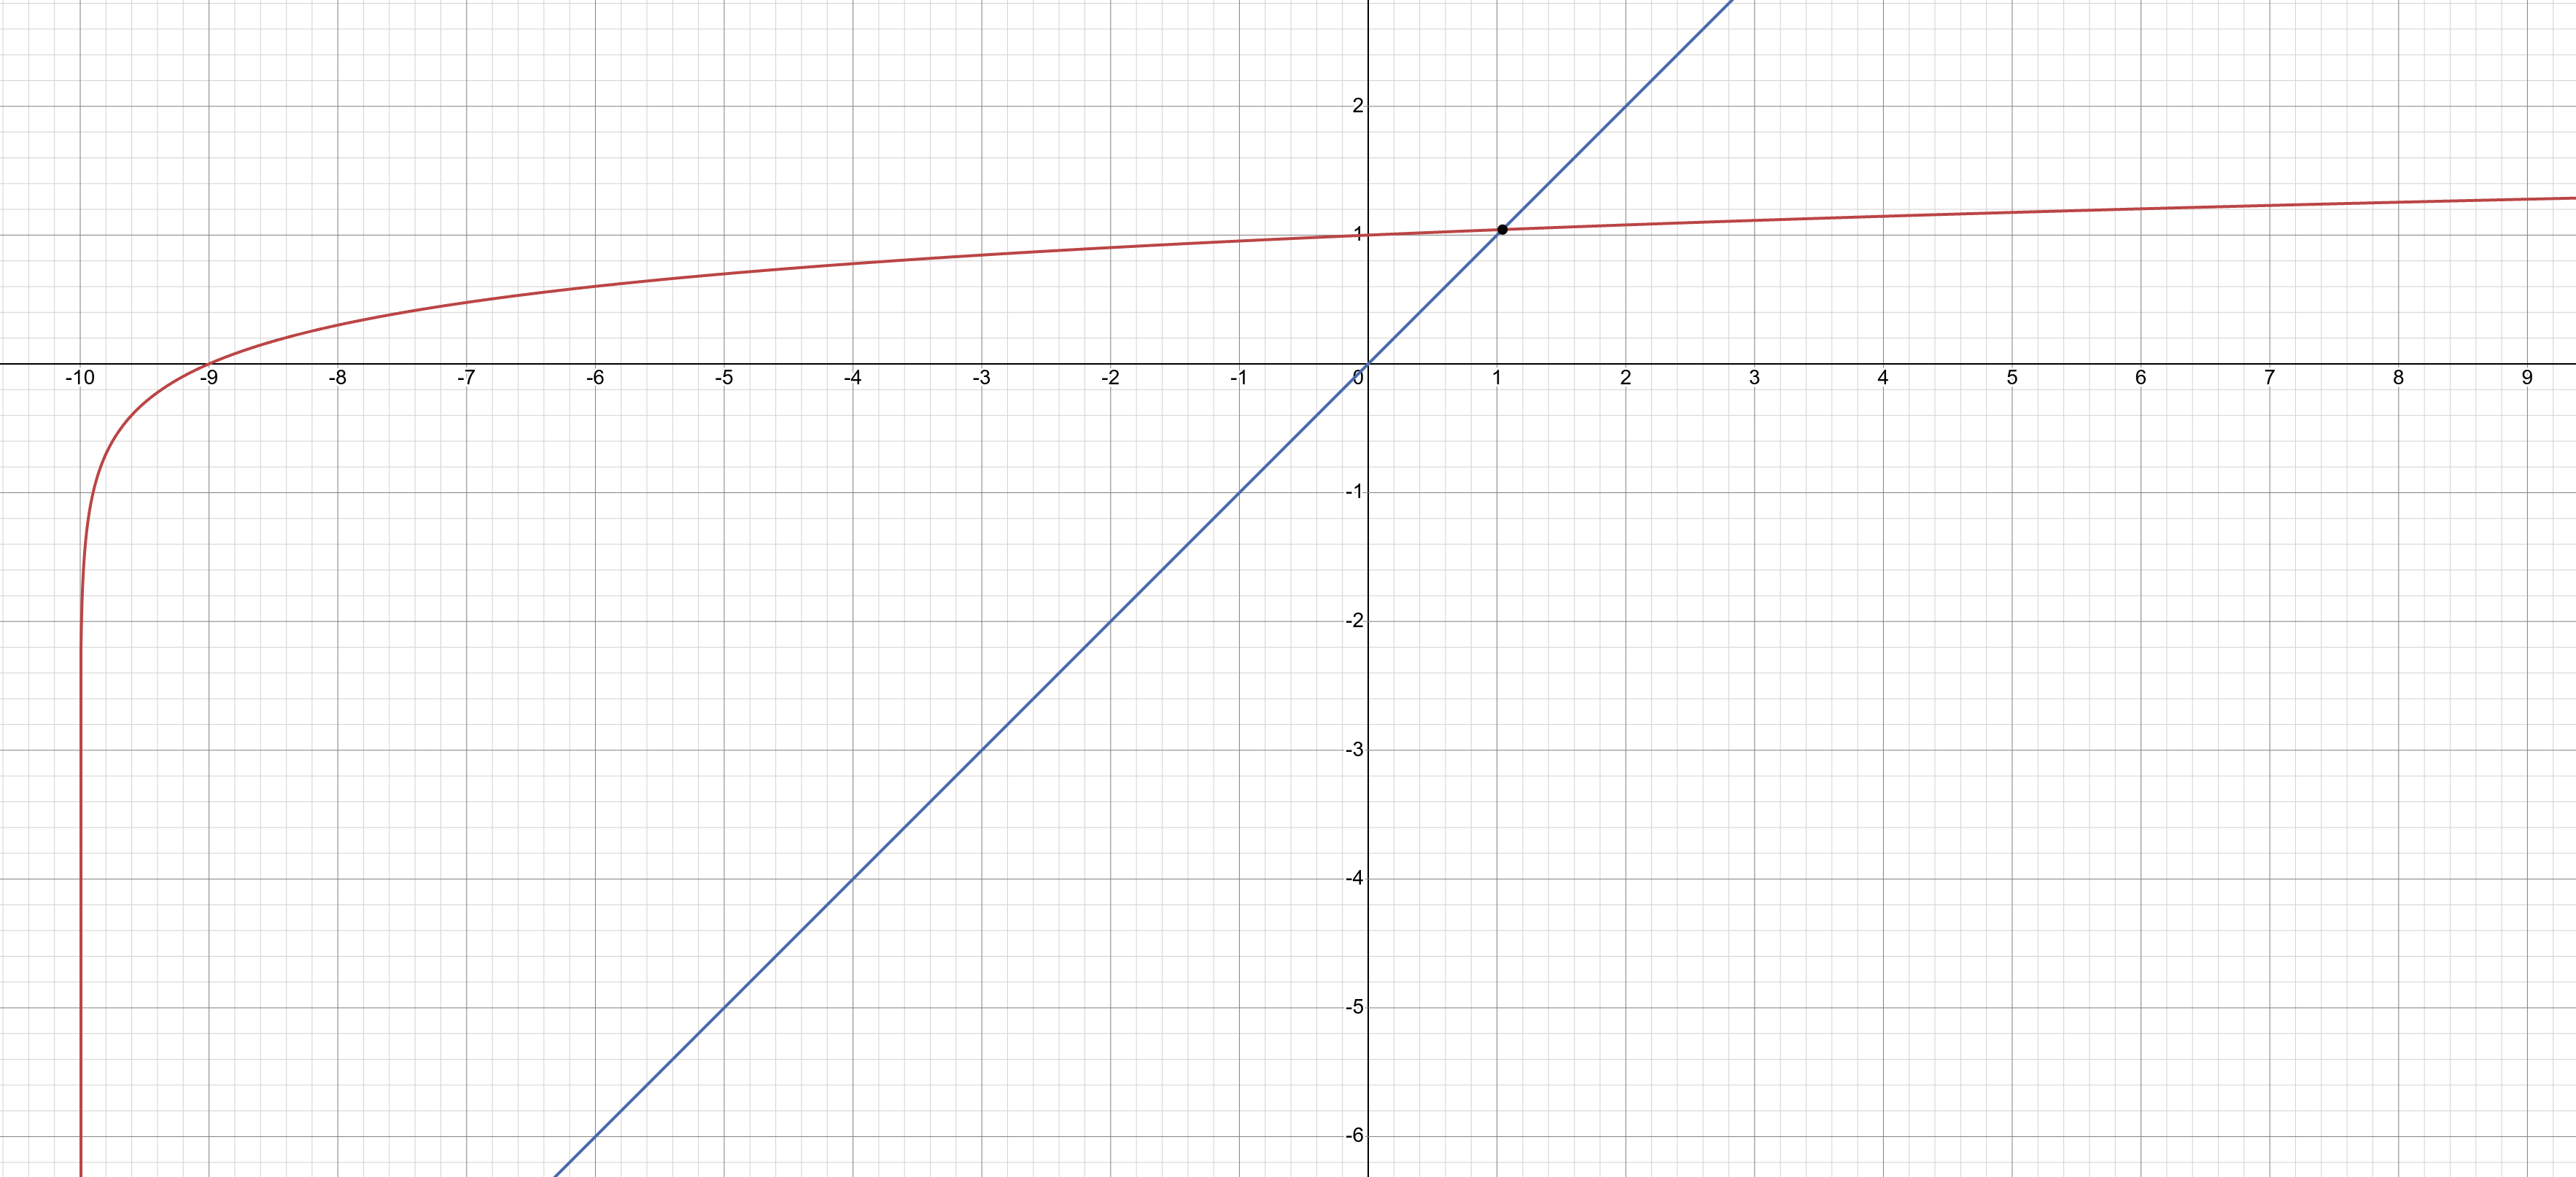
\includegraphics[height=1.3in,width=2.0in,viewport=0 0 2500 1600,clip]{Figures/solve_lg10.png}
%\caption{\tiny \textrm{The comparison of parallel scaling for ABINIT vs VASP.}}%(与文献\cite{EPJB33-47_2003}图1对比)
\label{solution-log_10}
\end{figure}
\end{minipage}
}

\frame[allowframebreaks]
{
	\frametitle{电荷密度混合收敛算法}
	根据\textrm{DFT},搜索基态电荷密度的过程就是能量泛函优化的过程,可以通过此前讨论的迭代算法实现:\\
%由初猜电荷密度出发,
	\begin{displaymath}
		R[\rho_{\mathrm{in}}]=\rho_{\mathrm{out}}[\rho_{\mathrm{in}}]-\rho_{\mathrm{in}}
	\end{displaymath}
	自洽迭代收敛时,残矢模量$\langle R[\rho_{\mathrm{in}}]|R[\rho_{\mathrm{in}}]\rangle~\rightarrow~0$

	\begin{itemize}
		\item 线性混合:\\
			如果电荷密度自洽迭代的每一步只保留当前步的电荷密度信息,就是线性电荷密度的线性混合
			\begin{displaymath}
				\rho_{\mathrm{in}}^{m+1}=\rho_{\mathrm{in}}^{m}+\gamma R[\rho_{\mathrm{in}}^m]
			\end{displaymath}
	显然,这种线性混合收敛比较慢,应用\textrm{Jacobian}矩阵相关的知识,通过选择\textrm{Preconditioning~}函数,加速自洽迭代的收敛
	\begin{displaymath}
		\rho_{\mathrm{in}}^{m+1}=\rho_{\mathrm{in}}^{m}+\mathbf{G}^1R[\rho_{\mathrm{in}}^m]
	\end{displaymath}
		\item \textrm{Kerker~}混合:\\%~
			以平面波为基,选择的\textrm{Preconditioning~}函数为
			\begin{displaymath}
				G_q^1=A\dfrac{q^2}{q^2+q_0^2}\quad\mbox{一般取$A=0.8$,$q_0$则可根据体系优化}
			\end{displaymath}
		\item \textrm{Pulay}混合:\\
			优化过程中,保留此前若干步的输入电荷密度和残矢,用于迭代的优化电荷密度由此前的电荷密度线性组合得到
			\begin{displaymath}
				\rho_{\mathrm{in}}^{\mathrm{opt}}=\sum_i\alpha_i\rho_{\mathrm{in}}^i
			\end{displaymath}
			\textcolor{magenta}{假设残矢与密度有相同的线性化形式}
			\begin{displaymath}
				R[\rho_{\mathrm{in}}^{\mathrm{opt}}]=R\bigg[\sum_i\alpha_i\rho_{\mathrm{in}}^i\bigg]=\sum_i\alpha_iR[\rho_{\mathrm{in}}^i]
			\end{displaymath}
			在归一化约束条件$\sum\limits_{i}\alpha_i=1$下,通过最小化残矢模量$\langle R\big[\rho_{\mathrm{in}}^{\mathrm{opt}}\big]|R\big[\rho_{\mathrm{in}}^{\mathrm{opt}}\big]\rangle$,得到优化电荷密度,可以得到优化系数$\alpha_i$
	\begin{displaymath}
		a_i=\dfrac{\sum\limits_{j}A_{j,i}^{-1}}{\sum\limits_{j,k}A_{j,k}^{-1}}\qquad A_{j,k}=\langle R[\rho_{\mathrm{in}}^{j}]|R[\rho_{\mathrm{in}}^{k}]\rangle 
	\end{displaymath}
\item \textrm{Brondey}混合:\\
	这是所有自洽求解\textrm{Kohn-Sham}方程方法中最复杂的,属于准-\textrm{Newton}类方法。在迭代过程中,用近似方法不断对\textrm{Jacobian~}矩阵(或逆矩阵)逼近\\
	每次自洽迭代中并不需要保存全部$N\times N$的\textrm{Jacobian}矩阵,只需要存储$N$-维矢量\\
	\textcolor{purple}{残矢可以线性化地表示为}
	\begin{displaymath}
		R[\rho]=R[\rho_{\mathrm{in}}^m]-\mathrm{J}^m(\rho-\rho_{\mathrm{in}}^m)
	\end{displaymath}
	这里$\mathbf{J}^m$是对\textrm{Jacobian~}矩阵的近似($(\mathbf{J}^m)^{-1}$是\textrm{Jacobian}矩阵的逆阵,习惯上取$\mathbf{G}^m=(\mathbf{J}^m)^{-1}$),由此可有迭代电荷密度
	\begin{displaymath}
		\rho_{\mathrm{in}}^{m+1}=\rho_{\mathrm{in}}^m+(\mathbf{J}^m)^{-1}R[\rho_{\mathrm{in}}^m]
	\end{displaymath}
	此类方法因为迭代中$\mathbf{J}^m$的变化形式不同,可以选择多种方案\\
	定义误差函数
	\begin{displaymath}
		E=w_0||\mathbf{G}^{m+1}-\mathbf{G}^m||^2+\sum_{i=1}^mw_i||\Delta\rho^i+\mathbf{G}^{m+1}\Delta R^i||^2
	\end{displaymath}
	这里$||A||^2=\langle A|A\rangle$,$w_i$是权重因子,并且有
	\begin{displaymath}
		\begin{aligned}
			\Delta\rho^i=&\rho_{\mathrm{in}}^{i+1}-\rho_{\mathrm{in}}^{i}\\
			\Delta R[\rho^i]=&R[\rho_{\mathrm{in}}^{i+1}]-R[\rho_{\mathrm{in}}^{i}]
		\end{aligned}
	\end{displaymath}
	\begin{itemize}
		\item 误差函数的第一项要求\textrm{Jacobian}矩阵的逆阵在迭代中变化不大,并有$w_0\rightarrow0$
		\item 误差函数的第二项要求模$||\Delta\rho^i+\mathbf{G}^{m+1}\Delta R^i||$足够小
	\end{itemize}
	用最小二乘法确定最小化误差,可以确定$\mathbf{G}^m$
	\begin{displaymath}
		\mathbf{G}^{m+1}=\mathrm{G}^1-\sum_{k=1}^m|\mathbf{Z}_k^m\rangle\langle\Delta R^k|
	\end{displaymath}
	其中
	\begin{displaymath}
		\begin{aligned}
			|\mathbf{Z}_k^m\rangle=&\sum_{n=1}^m\beta_{kn}w_kw_n|u^n\rangle+\sum_{n=1}^{m-1}\bar{\beta}_{kn}|\mathbf{Z}_n^{m-1}\rangle\\
			|u^n\rangle=&\mathbf{G}^1|\Delta R^n\rangle+|\Delta \rho^n\rangle
		\end{aligned}
	\end{displaymath}
	而$\beta_{kn}$和$\bar\beta_{kn}$由下式给出
	\begin{displaymath}
		\begin{aligned}
			\beta_{kn}=&\big(w_0^2+\bar A\big)_{kn}^{-1},\qquad \bar A_{kn}=w_kw_n\langle\Delta R^n|\Delta R^k\rangle\\
			\bar\beta_{kn}=&\delta_{kn}-\sum_{j=1}^mw_kw_j\beta_{kj}\langle\Delta R^n|\Delta R^j\rangle
		\end{aligned}
	\end{displaymath}
		{\fontsize{7.2pt}{4.2pt}\selectfont{
	不难看出\\$w_0\rightarrow 0$并且$w_0\ll w_n$,该方法就得到\textrm{Pulay}方法\\
	而一旦$w_0\rightarrow 0$时,$w_n$的选择,完全不会影响$\mathbf{G}^{m+1}$,因此取$w_n=1$可有
	\begin{displaymath}
		\mathbf{G}^m=\mathbf{G}^1-\sum_{k,n=1}^{m-1}\beta_{kn}|u^n\rangle\langle\Delta R^k|
	\end{displaymath}
而如果令$w_i=0$并要求$w_0\ll w_m$,有
\begin{displaymath}
	\begin{aligned}
		|\mathbf{Z}_k^m\rangle=&|\mathbf{Z}_k^{m-1}\rangle\qquad k<m\\
		|\mathbf{Z}_m^m\rangle=&\dfrac1{||\Delta R^m||^2}\bigg(|u^m\rangle-\sum_{k=1}^{m-1}\langle\Delta R^k|\Delta R^m\rangle|\mathbf{Z}_k^{m-1}\rangle\bigg)
	\end{aligned}
\end{displaymath}
}}
	\end{itemize}
}

\frame
{
	\frametitle{矩阵迭代对角化的基本思想}
\begin{figure}[h!]
\centering
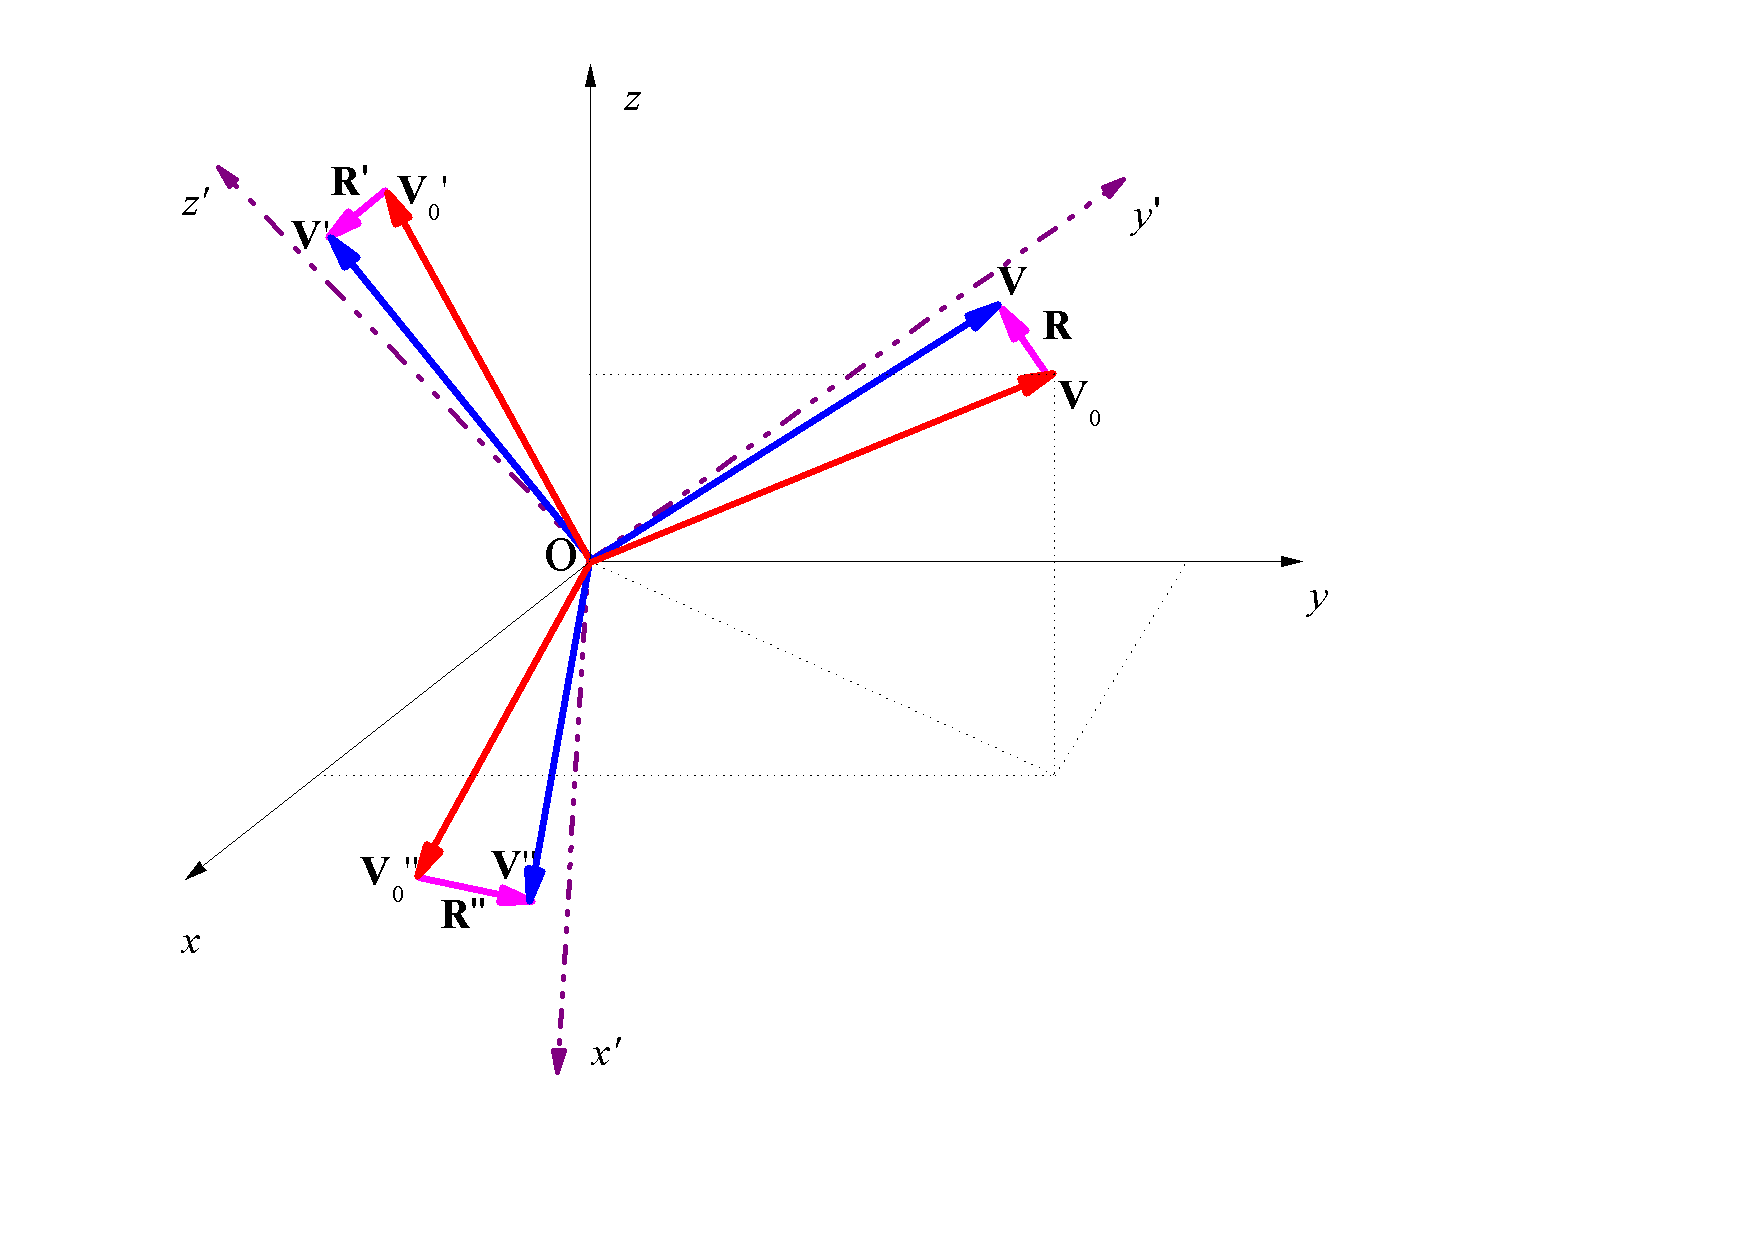
\includegraphics[height=2.5in,width=3.5in,viewport=0 0 850 590,clip]{Figures/Coordinate_transformation.png}
\label{decent_CG}
\caption{\tiny \textrm{Schematic illustration of searching for the eigenvalue of a vector.}}%(与文献\cite{EPJB33-47_2003}图1对比)
\end{figure}
}

\frame
{
	\frametitle{矩阵的迭代对角化}
	``预处理矩阵''$\mathbf{K}$的作用,是使\textcolor{red}{函数(泛函)对变量的依赖趋于“同质”(\textrm{isotropic})},即函数曲线与不同变量的依赖关系趋同

	具体到电子结构求解:~
	\begin{itemize}
		\item \textcolor{blue}{平面波基}\\
			基函数$\mathrm{e}^{\mathrm{i}\vec G_m\cdot\vec r}$对波函数$\psi_{\vec k_i+\vec G}^n(\vec r)$的贡献为$c_{i,m}^n(\vec k)$\\
		{\fontsize{7.2pt}{4.2pt}\selectfont{
		在能量泛函表达式中,高频(大的$\vec G_m$)部分比低频(小的$\vec G_m$)贡献大得多}}\\
			\textrm{preconditioning}\textcolor{blue}{要使不同频率对能量泛函贡献趋同}:\\
			\textcolor{red}{不同本征矢的修正项趋同,而与相应的能量本征值无关。}取
	\begin{displaymath}
		K(x)=\dfrac{27+18x+12x^2+8x^3}{27+18x+12x^2+8x^3+16x^4}
	\end{displaymath}
	此处定义
	\begin{displaymath}
		x_i^n(\vec G_m)=\dfrac12\dfrac{|\vec k+\vec G_m|^2}{E^{\mathrm{kin}}(\mathbf{R}^n)}
	\end{displaymath}
	\textcolor{purple}{$x_i^n(\vec G_m)$表示对$n$次迭代后本征态$i$中平面波组分$|\vec k_i+\vec G_m|$动能贡献的调整比例}
	\end{itemize}
}

\frame
{
	\frametitle{矩阵的迭代对角化}
	\begin{itemize}
		\item \textcolor{blue}{实空间基}\\
		与平面波基类似,可以定义
	\begin{displaymath}
		x_i^n(\vec r)=A\dfrac12\dfrac{\lambda_i^m-V(\vec r)}{E^{\mathrm{kin}}(\mathbf{R}^n)}
	\end{displaymath}
		\textcolor{purple}{$x_i^n(\vec r)$表示对$n$次迭代后本征态$i$中局部动能$|\lambda_i-V(\vec r)|$对总动能贡献的调整比例}
	\end{itemize}
	完成\textrm{preconditioning}得到矩阵$\mathbf{K}(x_i^n)$后,由
	\begin{displaymath}
		\psi^{n+1}\equiv\mathbf{K}\mathbf{R}^n
	\end{displaymath}
	可根据残矢量$\mathbf{R}^n$选择方式的不同,将\textcolor{blue}{\textrm{SD}、\textrm{CG}}、\textcolor{blue}{\textrm{RMM-DIIS}}等多种算法应用于矩阵迭代对角化计算
}

\subsection{经典分子动力学提要}
\frame
{
	\frametitle{经典分子动力学}
	装有$N$个经典粒子的$L_1\times L_2\times L_3$容器内,假设粒子间只有简单的二体相互作用\footnote{\fontsize{7.2pt}{6.2pt}\selectfont{二体作用是粒子间多体相互作用的简化,只考虑粒子两两间彼此相互作用。}}$\vec F(r)$,力的大小仅与粒子间间距$r$相关
	\begin{displaymath}
		\vec F(R_i)=\sum_{\substack{j=1\\j\neq i}}^N F(|\vec r_i-\vec r_j|)\hat{\vec r}_{ij}
	\end{displaymath}
	{\fontsize{7.2pt}{6.2pt}\selectfont{这里$R$代表全部原子坐标$\vec r_i$,$\hat{\vec r}_{ij}$是表示粒子$i$指向粒子$j$的矢量($\vec r_j-\vec r_i$)的单位矢量}}

	在经典力学框架下,粒子$i$的受力运动方程是:~
	\begin{displaymath}
		\dfrac{\mathrm{d}^2\vec r_i(t)}{\mathrm{d}t^2}=\dfrac{\vec F_i(R)}{m_i}
	\end{displaymath}
	粒子$i$的质量是$m_i$\\
	\textcolor{purple}{经典分子动力学,就是应用数值模拟对大量粒子求解该方程,基于统计力学原理,研究物质的状态和热力学性质}
}

\frame
{
	\frametitle{经典分子动力学与\textrm{Verlet}算法}
	分子动力学模拟研究的对象是平衡态体系
	\begin{itemize}
		\item 初始化
		\item 开始分子运动模拟,直到模拟体系达到平衡
		\item 继续模拟体系的物理性质,保存计算结果
	\end{itemize}
	\textcolor{blue}{标准\textrm{Verlet}算法:~}求解作用力$\vec F$下单个粒子运动的积分
	\begin{displaymath}
		\vec r(t+h)=2\vec r(t)-\vec r(t-h)+h^2\vec F(\vec r(t))/m
	\end{displaymath}
	{\fontsize{7.2pt}{6.2pt}\selectfont{这里$h$是时间步长,$t=nh$是模拟累积时间,$\vec r(t)$是粒子在时间$t$时的位置\\
	\textcolor{magenta}{每个时间步长的误差为$h^4$,在模拟时间范围内的累积误差是$h^2$}
\vskip 5pt
	{\fontsize{7.2pt}{6.2pt}\selectfont{如果已知模拟粒子的初始速度$\vec v$和时间,取初始态时间$t=0$}}
	\begin{displaymath}
		\vec r(h)=\vec r(0)=h\vec v(0)+\dfrac{h^2}2\vec F[\vec r(t=0)]~\qquad~ (m\equiv1)
	\end{displaymath}
误差为$h^3$,速度随时间变化的函数
\begin{displaymath}
	\vec v(t)=\dfrac{\vec r(t+h)-\vec r(t-h)}{2h}+\mathscr{O}(h^2)
\end{displaymath}
}}
}

\frame
{
	\frametitle{经典分子动力学与\textrm{Verlet}算法}
	\textrm{Verlet}算法有两种被普遍应用的变体形式,相比于标准\textrm{Verlet}算法,这两种方法误差累积效应更小
	\begin{itemize}
		\item \textcolor{blue}{蛙跳(\textrm{Leap-Frog})法}
			\begin{displaymath}
				\begin{aligned}
					\vec v(t+h/2)=&\vec v(t-h/2)+h\vec F[\vec r(t)]\\
					\vec r(t+h)=&\vec r(t)+h\vec v(t+h/2)
				\end{aligned}
			\end{displaymath}
		\item \textcolor{blue}{速度-\textrm{Verlet}算法}
			\begin{displaymath}
				\vec v(t)=\dfrac{\vec r(t+h)-\vec r(t-h)}{2h}
			\end{displaymath}
			\begin{displaymath}
				\begin{aligned}
					\vec r(t+h)=&\vec r(t)+h\vec v(t)+h^2\vec F(t)/2\\
					\vec v(r+h)=&\vec v(t)+h[\vec F(t+h)+\vec F(t)]/2
				\end{aligned}
			\end{displaymath}
			速度-\textrm{Verlet}算法更稳定也更方便,但需要保存$\vec F(t)$和$\vec F(t+h)$两个力的数组
	\end{itemize}
}

\frame
{
	\frametitle{经典分子动力学与\textrm{Verlet}算法}
	以下算法与速度-\textrm{Verlet}算法完全等价,但只需要保留$\vec F(t)$一个数组
	\begin{displaymath}
		\begin{aligned}
			\tilde{\vec v}(t)=&\vec v(t)+h\vec F(t)/2\\
			\vec r(t+h)=&\vec r(t)+h\tilde{\vec v}(t)\\
			\vec v(t+h)=&\tilde{\vec v}(t)+h\vec F(t+h)/2
		\end{aligned}
	\end{displaymath}
	而粒子受力$\vec F(t+h)$则在第二步、第三步之间临时计算
\vskip 5pt
	{\fontsize{6.2pt}{4.2pt}\selectfont{一般地,作用在粒子$i$上的力,是所有与粒子$i$的相互作用的“合成”结果
	\begin{displaymath}
		\vec F_i(R)=-\dfrac{\partial U(\{\vec r_i\})}{\partial \vec r_i}
	\end{displaymath}
	通常总的势能$U(\{\vec r_i\})$拆解为各部分贡献
	\begin{displaymath}
		U(\{\vec r_i\})=\sum_iU_1(\vec r_i)+\sum_i\sum_{j>i}U_2(\vec r_i,\vec r_j)+\sum_i\sum_{j>i}\sum_{k>j}U_3(\vec r_i,\vec r_j,\vec r_k)+\cdots
	\end{displaymath}
	这里$U_1(\vec r_i)$是单体势,一般是单个粒子在外场(如重力场、电场)中的势能,与材料性质无关\\
$U_2(\vec r_i,\vec r_j)$是双体势,$U_3(\vec r_i,\vec r_j,\vec r_k)$是描述粒子间对相互作用的主要函数}}

	在分子动力学计算中,力的计算需要更多的时间,因为其计算耗时步数是$\mathscr{O}(N^2)$,\textcolor{blue}{对于周期体系,这种力的计算尤其需要谨慎}
}

\frame[allowframebreaks]
{
	\frametitle{经典分子动力学力场}
	原子间受力一般用\textcolor{red}{力场}(\textrm{Force Field},也就是“\textcolor{blue}{相互作用势}”)描述,力场的形式有很多种,典型力场的有
	\begin{itemize}
		\item \textrm{Lennard-Jones}对势
	\begin{displaymath}
		U(r)=4\varepsilon\bigg[\bigg(\dfrac{\sigma}{r}\bigg)^{12}-\bigg(\dfrac{\sigma}{r}\bigg)^6\bigg]
	\end{displaymath}
	{\fontsize{7.2pt}{6.2pt}\selectfont{这里$\varepsilon$和$\sigma$是和原子有关的参数
	\textrm{L-J}势能的最低点在$r_{\min}=2^{(1/6)}\sigma\approx1.12\sigma$,$r<r_{\min}$时为排斥力,$r>r_{\min}$时为吸引力
\begin{figure}[h!]
\centering
\vspace*{-0.30in}
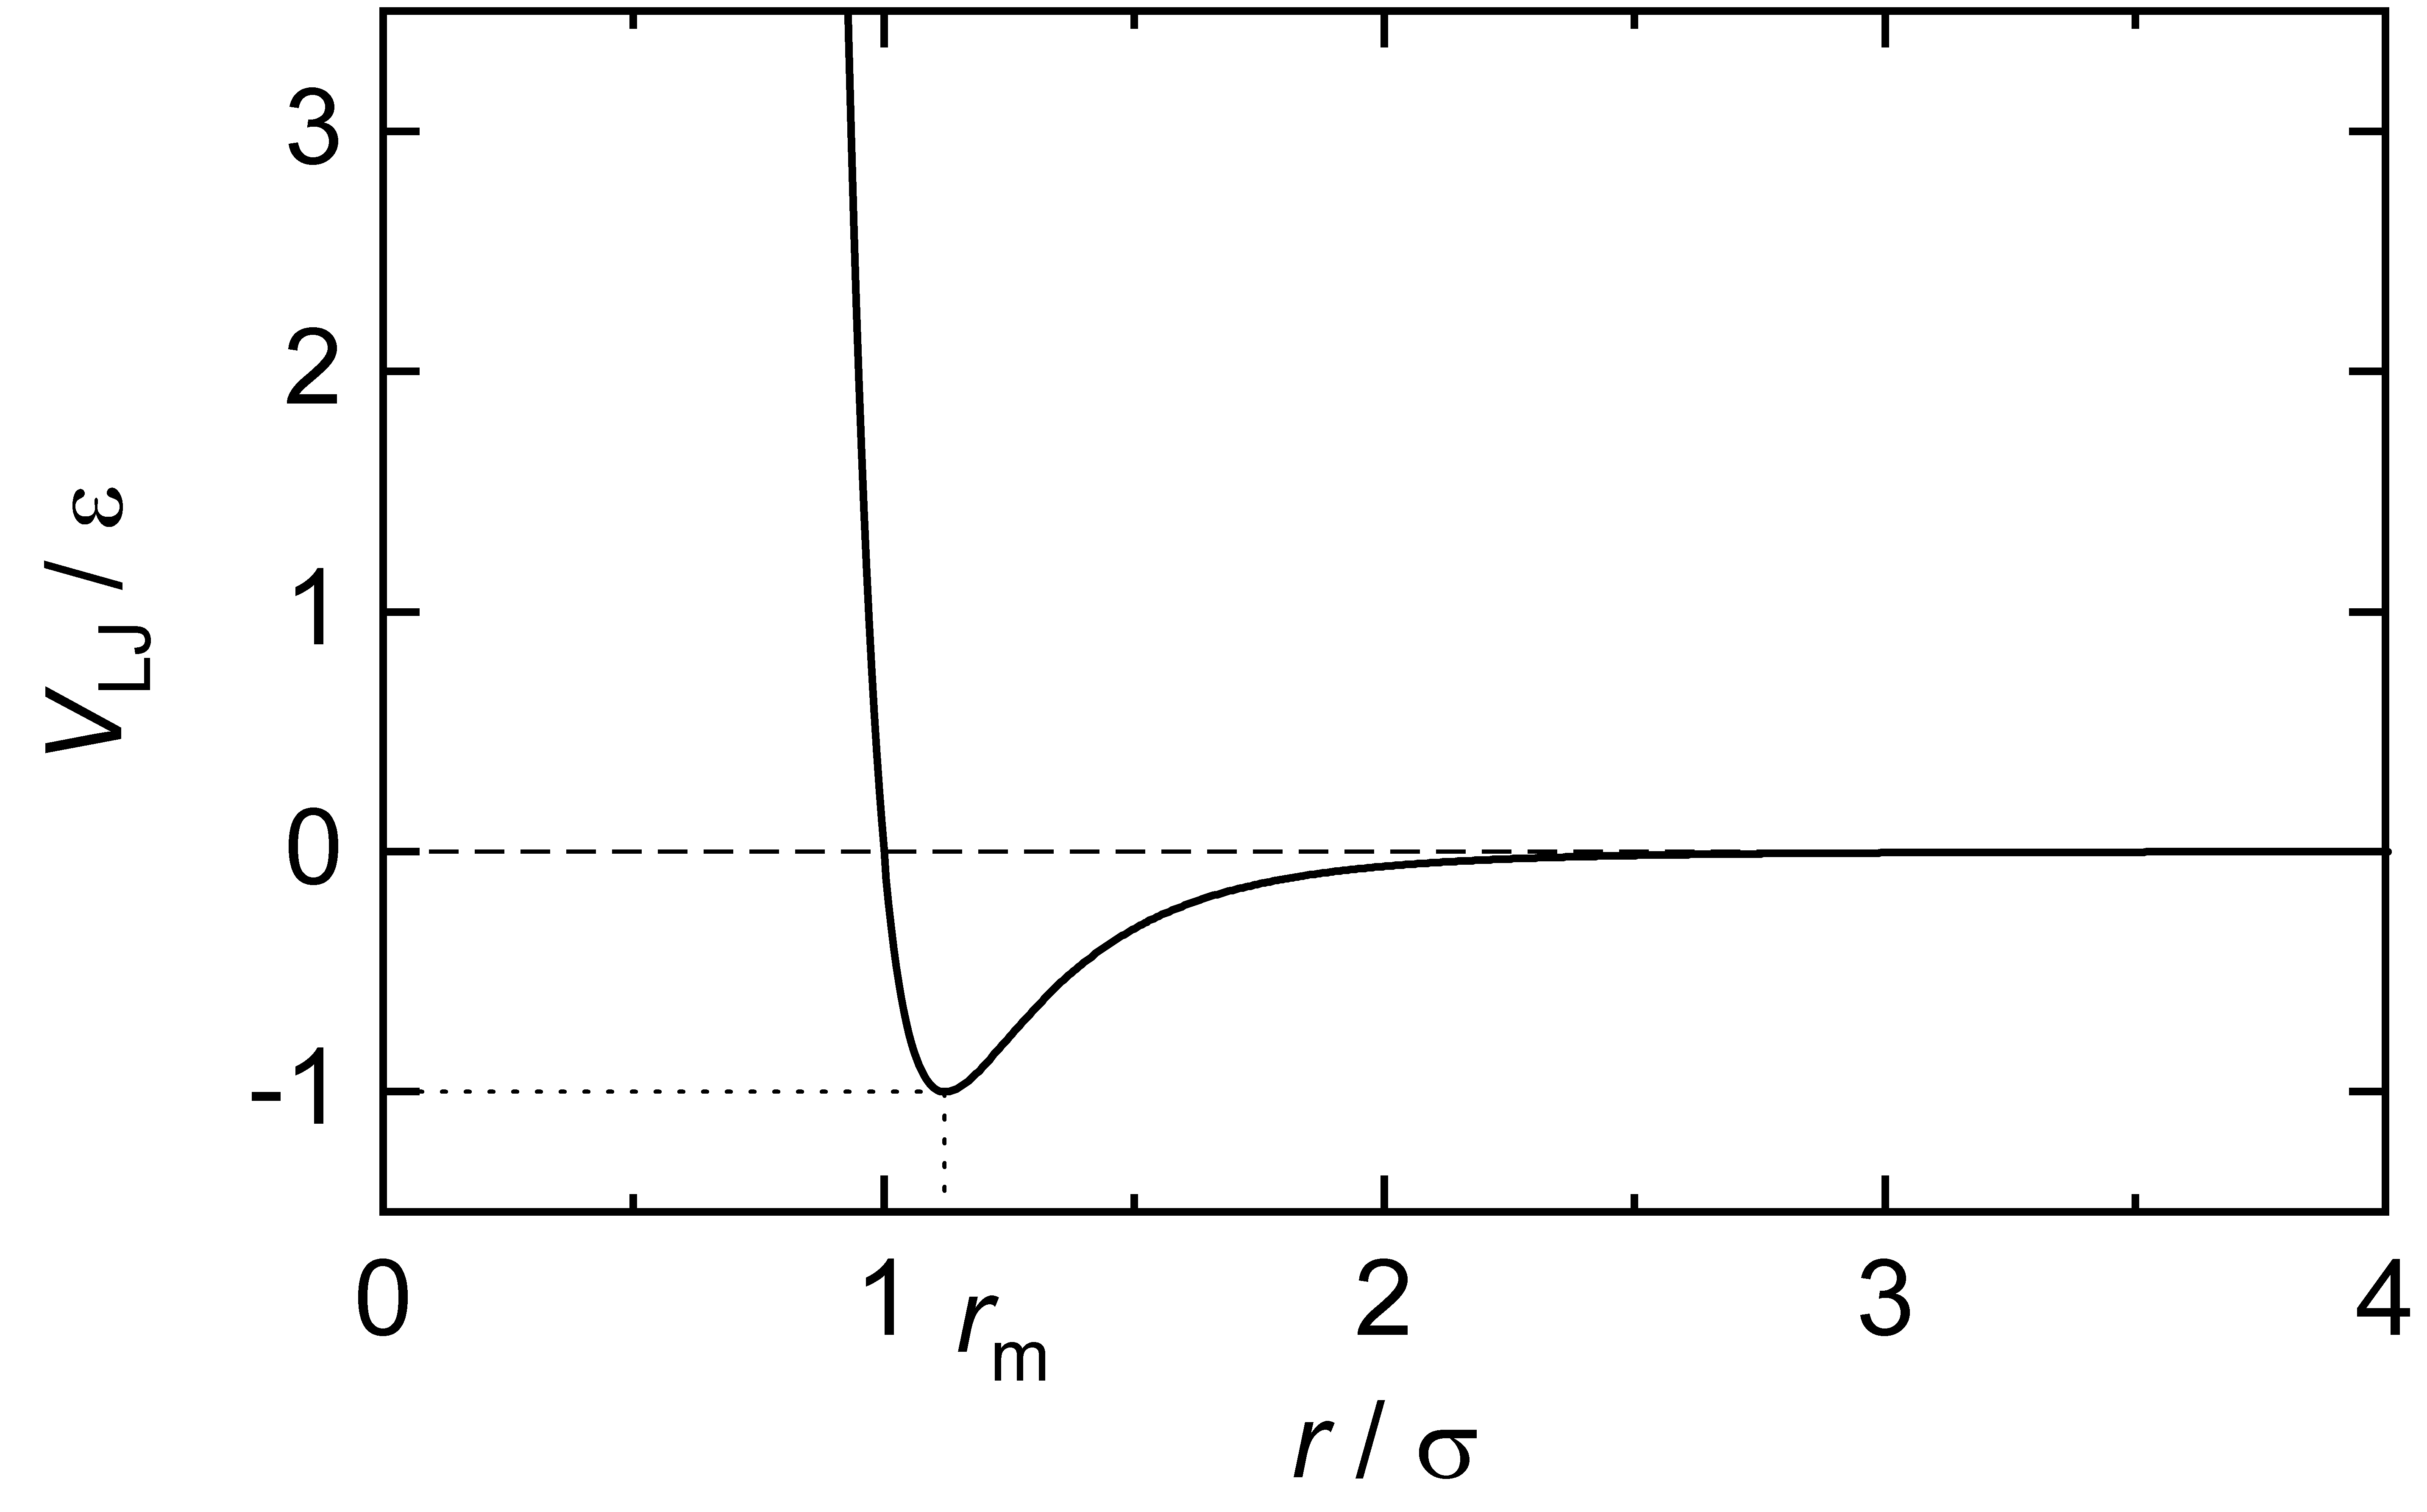
\includegraphics[height=1.00in,width=1.35in,viewport=0 0 340 270,clip]{Figures/Lennard-Jones_potential.png}
\caption{\tiny \textrm{The Lennard-Jones Potential.}}%(与文献\cite{EPJB33-47_2003}图1对比)
\label{Potential-Lennard-Jones}
\end{figure}
\vskip -20pt
	由\textrm{L-J}势改造,可以得到\textrm{WCA}势和\textrm{PHS}势}}
\item \textrm{Morse}势
	\begin{displaymath}
		U(r)=-D_{\mathrm{e}}+D_{\mathrm{e}}\bigg(1-\mathrm{e}^{-a(r-r_{\mathrm{e}})}\bigg)^2
	\end{displaymath}
	{\fontsize{7.2pt}{6.2pt}\selectfont{这里$D_{\mathrm{e}}$是\textrm{Morse}势的势阱深,参数$a$确定势阱宽度,$r_{\mathrm{e}}$是原子处于平衡位置的平衡键长
\begin{figure}[h!]
\centering
\vspace*{-0.15in}
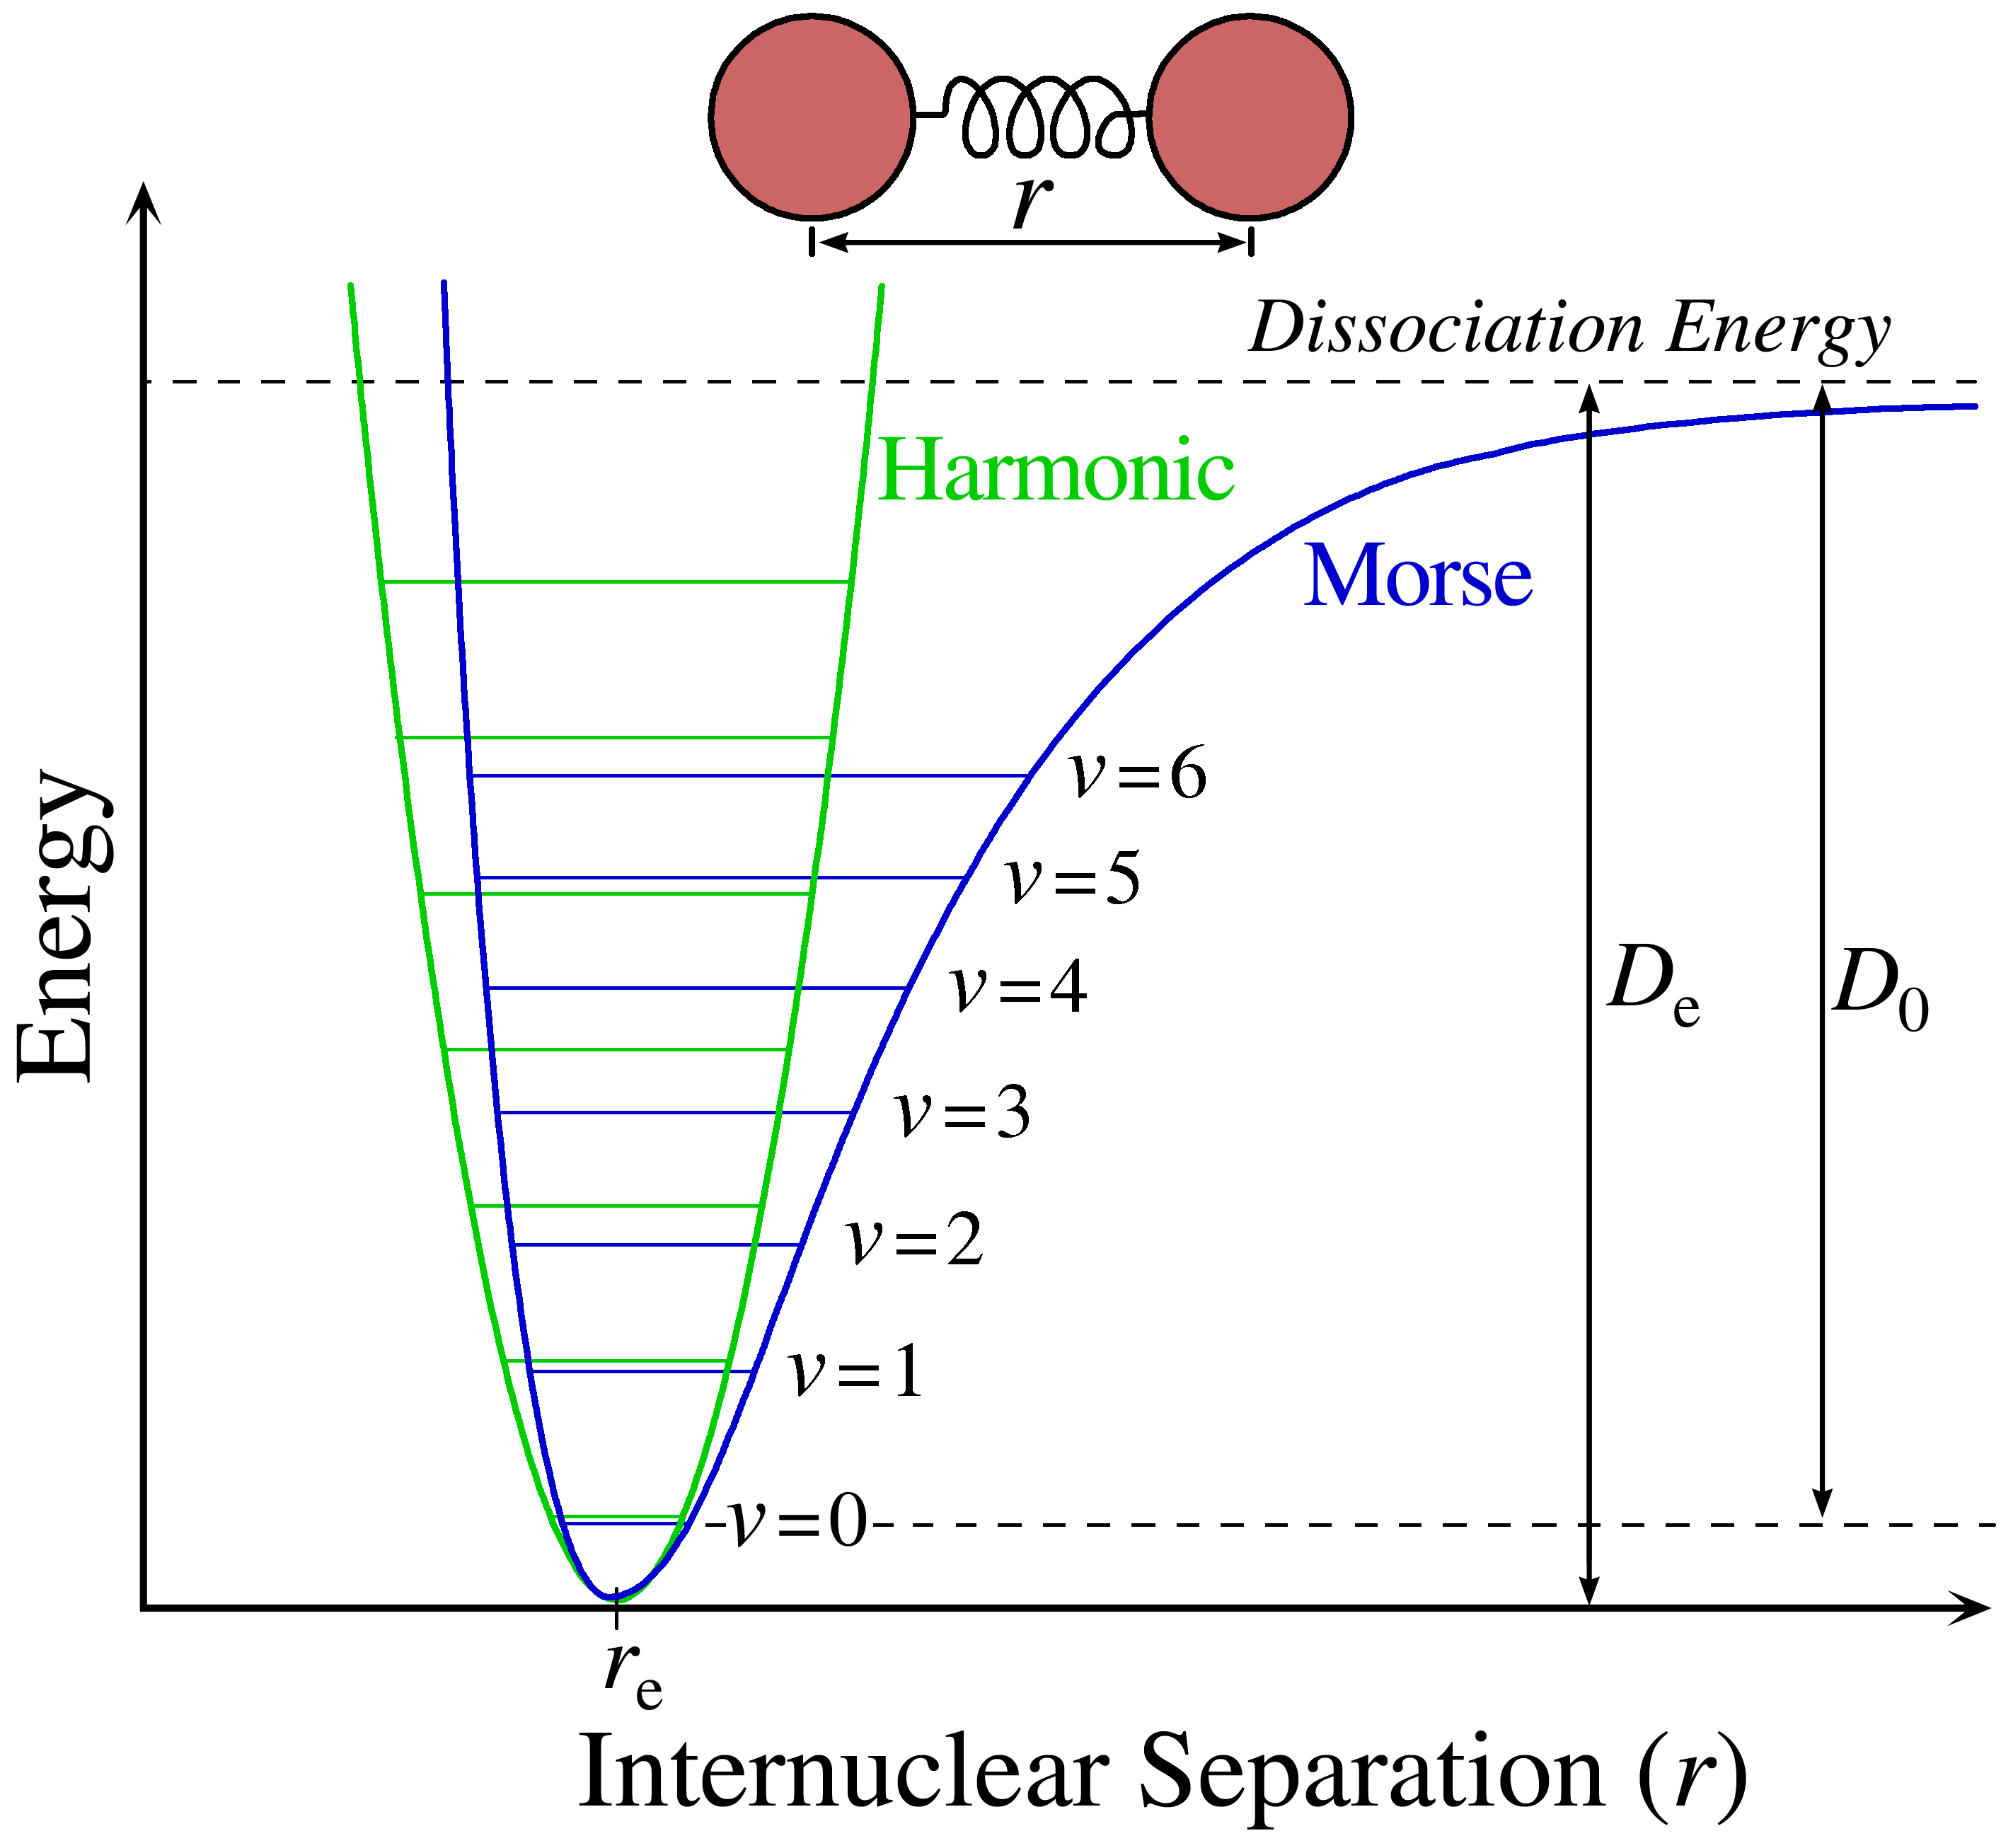
\includegraphics[height=1.30in,width=1.85in,viewport=0 0 3540 2770,clip]{Figures/Morse-potential.png}
\caption{\tiny \textrm{The Morse potential (blue) and harmonic oscillator potential (green).}}%(与文献\cite{EPJB33-47_2003}图1对比)
\label{Potential-Morse}
\end{figure}
}}
\item \textrm{EAM}势\\
	{\fontsize{7.2pt}{6.2pt}\selectfont{对于金属晶体,内能虽可以表示为对相互作用之和,但拟合原子受力非常困难:\footnote{\fontsize{5.2pt}{3.2pt}\selectfont{应用二体势计算金属弹性常数时必须涉及对体积很敏感的能量项,因为涉及缺陷、表面的体积很难确定。}}\\
	\textcolor{red}{从物理上说金属原子处于电子海洋中,电子密度来自多个原子的贡献,这是自由电子气带来的多体效应}}}\\
	\textrm{EAM}将金属中原子的势能表示为二体势和多体势之和
	\begin{displaymath}
		E_i=F_{\alpha}\bigg(\sum_{j\neq i}\rho_{\beta}(r_{ij})\bigg)+\dfrac12\sum_{j\neq i}\phi_{\alpha\beta}(\vec r_{ij})
	\end{displaymath}
	{\fontsize{7.2pt}{6.2pt}\selectfont{$\alpha$和$\beta$分别为位置$i$、$j$处的原子类型\\
		$\phi$是二体势,是原子$\alpha$和$\beta$和原子间距$r_{ij}$的函数\\
		$F$是多体势,是其余原子在位置$i$处的电荷密度与位置$i$处原子$\alpha$的相互作用能,由原子类型$\alpha$和位置$i$处的电子密度确定\\
		位置$j$原子在位置$i$处产生的电荷密度$\rho$只与位置$j$处原子类型$\beta$和原子间距$r_{ij}$有关,与方向无关
	}}\\
	各类\textrm{EAM}势中,$\phi(r)$、$\rho(r)$和$F(\rho)$都不是解析的,以数值形式存储
	\end{itemize}
}

\frame
{
	\frametitle{统计系综}
	系综(\textrm{Ensembles})是在一定的宏观条件下,由大量微观粒子组成的性质和结构完全相同的、处于各种运动状态的、各自独立的系统整体的集合\footnote{\fontsize{4.2pt}{2.2pt}\selectfont{简言之,系综是系统的集合(\textcolor{magenta}{系统}:~宏观相同,微观不同)。}}。\\
	应用\textrm{Verlet}算法,完成单粒子运动的数值积分,可以得到动力学体系的\textrm{Hamiltonian}对应的能量,进而应用统计力学的统计系综,获得宏观体系的物理量
\begin{figure}[h!]
\centering
\vspace*{-0.20in}
%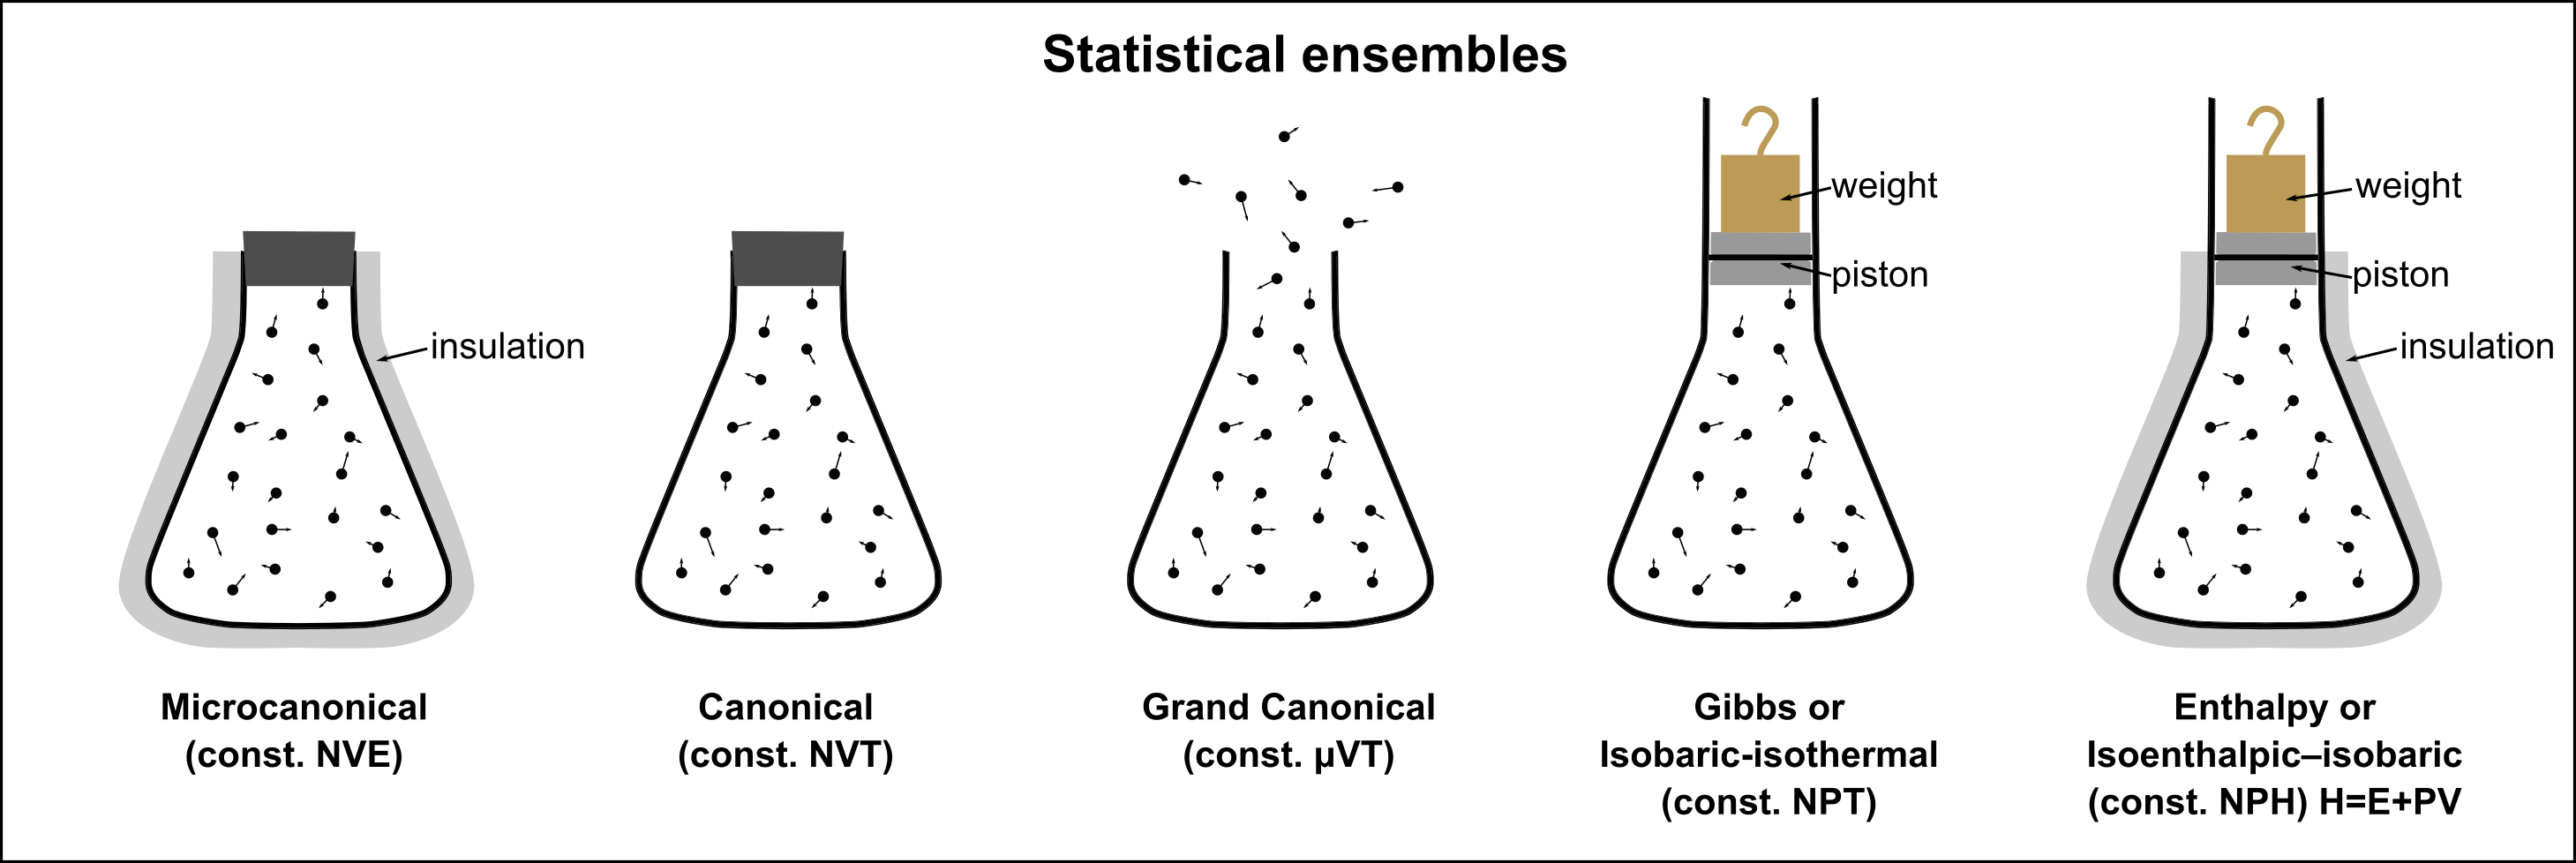
\includegraphics[height=1.60in,width=3.85in,viewport=0 0 1420 570,clip]{Figures/Statistical_Ensembles.png}
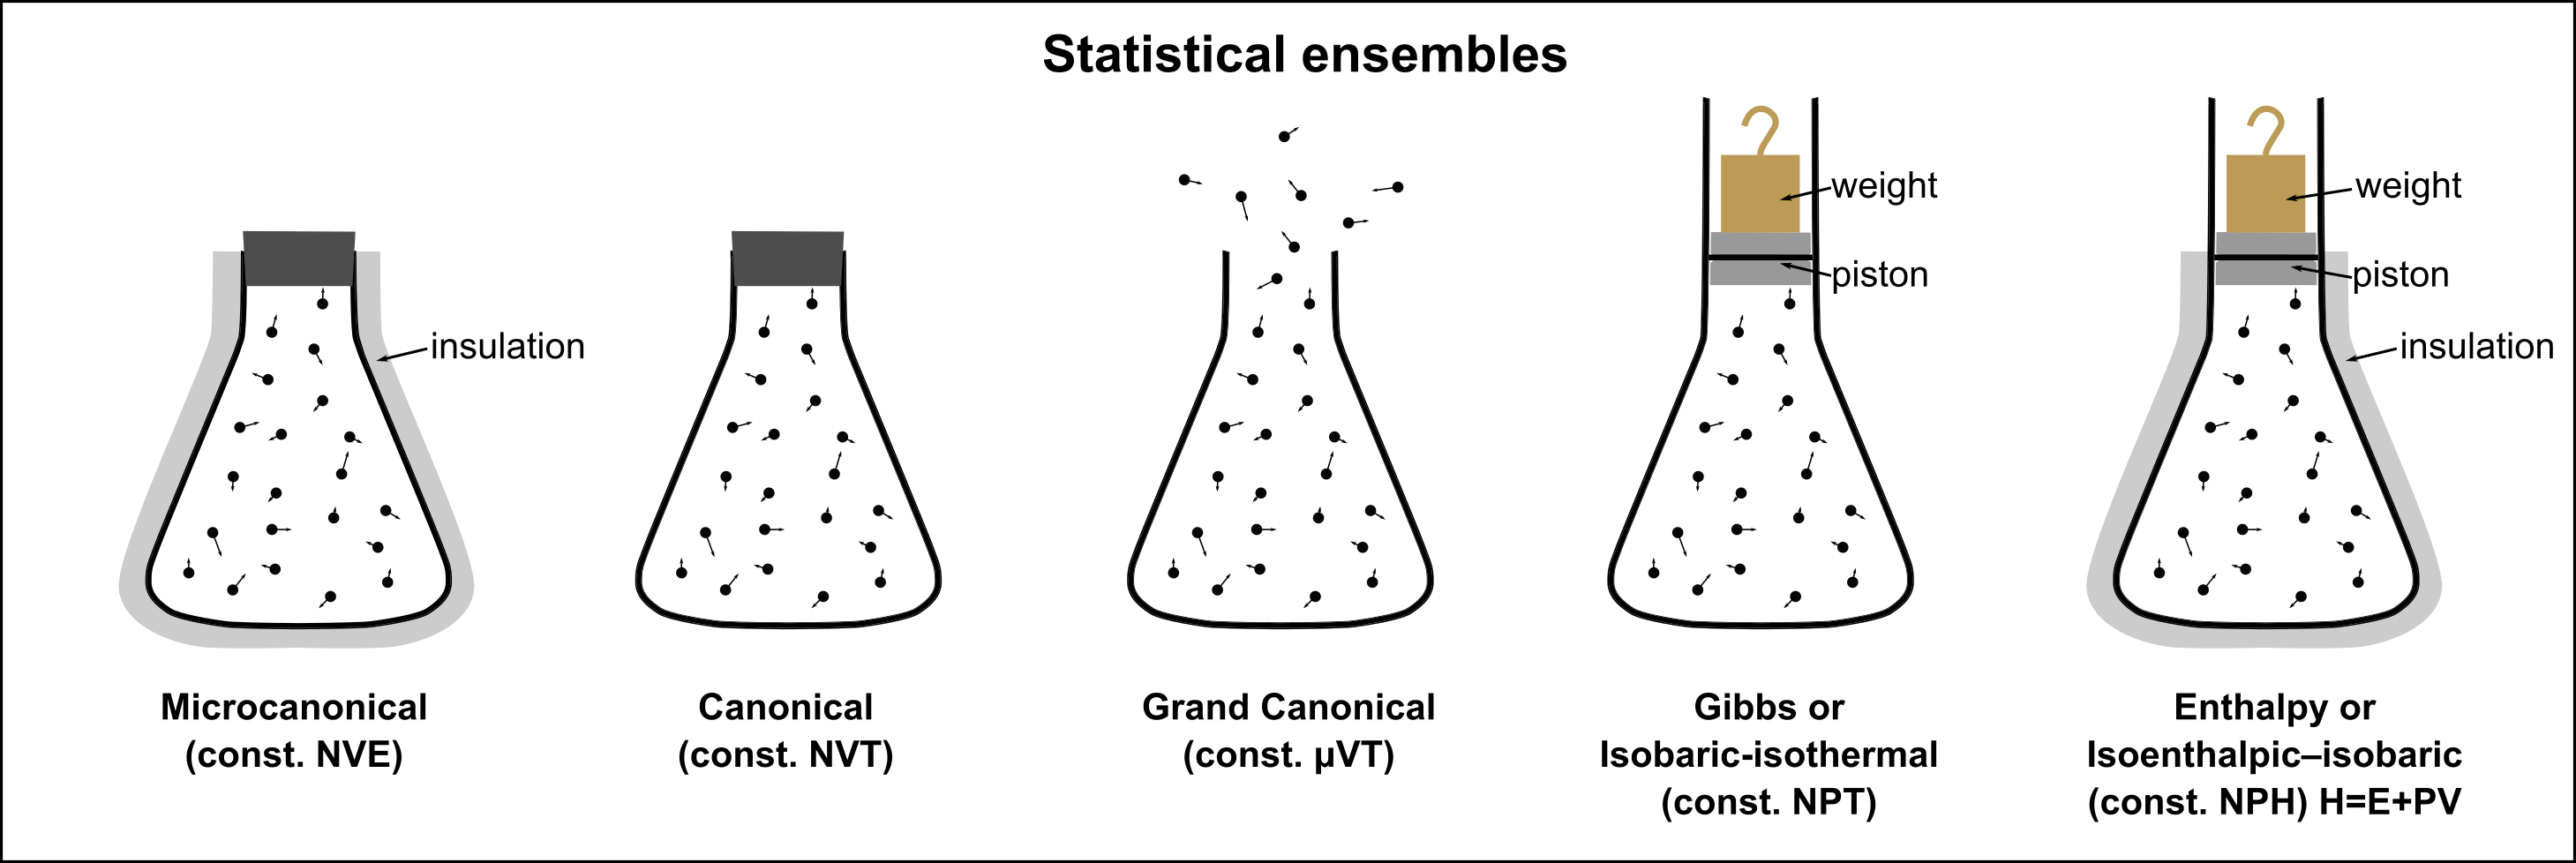
\includegraphics[height=1.30in,width=3.35in,viewport=0 0 1420 570,clip]{Figures/Statistical_Ensembles.png}
\caption{\tiny \textrm{The Statistical Ensembles.\footnote{\fontsize{3.5pt}{1.2pt}\selectfont{\textrm{canonical},汉译作“正则”,出自《楚辞\textperiodcentered 离骚》“皇揽揆余於初度兮,肇锡余以嘉名;~名余曰\textcolor{red}{正则}兮,字余曰灵均”,《楚辞章句》\upcite{Chucizhangju}:~“正,平也;~则,法也;~灵,神也;~均,调也。言正平可法则者,莫过于天;~养物均调者,莫过于地。高平曰原,故父伯庸名我为平以法天,字我为原以法地。言己上能安君,下能养民也。”,意思是说“正则”、“灵均”隐喻着某种意义,即平正是天的象征,原均是地的象征。因此正则的含义是“符合天道”,与\textrm{canonical}的意思\textrm{of, relating to, or forming a canon}意义一致。}}}}%(与文献\cite{EPJB33-47_2003}图1对比)
\label{Statistical_Ensembles}
\end{figure}
}

\subsection{第一原理分子动力学简介}
\frame
{
	\frametitle{第一原理分子动力学}
	电子结构计算时,体系总能是基于\textrm{Born-Oppenheimer}近似得到,如果变化原子位置,可以得到体系总能随原子位置变化的规律\\
	作为原子位置$\vec R_i$函数的电子态总能量$E(\vec R_1,\vec R_2,\cdots,\vec R_N)$称\textcolor{red}{势能面}~(\textrm{potential surface})

	对于一套给定原子核位置$\mathbf{S}=(\vec R_1,\cdots,\vec R_N)$,$\vec R_i$表示第$i$个原子核的位置;~如果电子的基态波函数是$\psi_{\mathrm{G}}$则\\电子态能量为
	\begin{displaymath}
		E=\dfrac{\langle\psi_{\mathrm{G}}|\mathbf{H}(\mathbf{S})|\psi_{\mathrm{G}}\rangle}{\langle\psi_{\mathrm{G}}|\psi_{\mathrm{G}}\rangle}
	\end{displaymath}
作用在原子核$n$上的经典作用力,可由电子态能量对原子位置$\vec R_n$的梯度$\nabla_n$的负值给出
\begin{displaymath}
	\vec F_n=-\nabla_nE(\mathbf{S})=-\nabla_n\bigg[\dfrac{\langle\psi_{\mathrm{G}}|\mathbf{H}(\mathbf{S})|\psi_{\mathrm{G}}\rangle}{\langle\psi_{\mathrm{G}}|\psi_{\mathrm{G}}\rangle}\bigg]
\end{displaymath}
}

\frame
{
	\frametitle{\textrm{Hellmann-Feynman}定理}
	如果$\psi_{\mathrm{G}}$是\textrm{Hamiltonian}的本征态,有
	\begin{displaymath}
		\begin{aligned}
			&(\langle\psi_{\mathrm{G}}|\psi_{\mathrm{G}}\rangle)^2\nabla_nE\\
			=&\big[\langle(\nabla_n\psi_{\mathrm{G}}|\mathbf{H}|\psi_{\mathrm{G}}\rangle+\langle\psi_{\mathrm{G}}|(\nabla_n\mathbf{H})|\psi_{\mathrm{G}}\rangle+\langle\psi_{\mathrm{G}}|\mathbf{H}|(\nabla_n\psi_{\mathrm{G}})\rangle\big]\langle\psi_{\mathrm{G}}|\psi_{\mathrm{G}}\rangle\\
			&-\langle\psi_{\mathrm{G}}|\mathbf{H}|\psi_{\mathrm{G}}\rangle\big[\langle(\nabla_n\psi_{\mathrm{G}})|\psi_{\mathrm{G}}\rangle+\langle\psi_{\mathrm{G}}|(\nabla_n\psi_{\mathrm{G}})\rangle\big]
		\end{aligned}
	\end{displaymath}
	{\fontsize{6.2pt}{5.2pt}\selectfont{这里暂不考虑$\mathbf{H}$对原子核位置$\mathbf{S}$的依赖}}\\
	\vskip 5pt
	\textrm{Hellmann-Feynman}定理指出:~如果\textrm{Hamiltonian}量$\mathbf{H}$是\textrm{Hermitian}的,并且有
	\begin{displaymath}
		\mathbf{H}\psi_{\mathrm{G}}=E_{\mathrm{G}}\psi_{\mathrm{G}}
	\end{displaymath}
则上述表达式中,除了$\langle\psi_{\mathrm{G}}|(\nabla_n\mathbf{H})|\psi_{\mathrm{G}}\rangle$之外,等式右侧其余各项彼此抵消。由此得到能量梯度的表达式
\begin{displaymath}
	\nabla_nE=\dfrac{\langle\psi_{\mathrm{G}}|(\nabla_n\mathbf{H})|\psi_{\mathrm{G}}\rangle}{\langle\psi_{\mathrm{G}}|\psi_{\mathrm{G}}\rangle}
\end{displaymath}
}

\frame
{
	\frametitle{\textrm{Car-Parrinello~}方法}
	基于\textrm{Born-Oppenheimer}近似的原子-电子耦合的势能面计算,因每一原子步都需要完整的电子结构自洽迭代,故计算量非常可观。
\vskip 5pt
\textrm{1985}年,在\textrm{Car-Parrinello}给出的方案中,\textcolor{purple}{电子态将和原子核的运动一样,都用分子动力学算法处理}\\
在该方案中,\textcolor{blue}{体系的电子态并未能达到当前正电荷环境的真实基态,但体系总能可以与真实基态更为接近}\\
{\fontsize{6.2pt}{5.2pt}\selectfont{考虑\textcolor{blue}{电子态总能}(即\textcolor{red}{电子态有关能量}+\textcolor{magenta}{原子核静电相互作用能})是作为电子波函数$\psi_k$和原子核坐标$\mathbf{S}$的泛函
\begin{displaymath}
	E_{\mathrm{tot}}=E_{\mathrm{tot}}(\{\psi_k\},\mathbf{S})
\end{displaymath}
如果波函数可用一套基组$\{\chi_r\}$表示,即
\begin{displaymath}
	\psi_k(\vec r)=\sum_rC_{rk}\chi_r(\vec r)
\end{displaymath}
则体系总能可表示为
\begin{displaymath}
	E_{\mathrm{tot}}=E_{\mathrm{tot}}(\{C_{rk}\},\mathbf{S})
\end{displaymath}
考虑到基函数常常选择以原子核为坐标原点,因此也依赖于$\mathbf{S}$
}}\\
\textrm{Car-Parrinello}方法通过变量\underline{\textcolor{blue}{$\psi_k$(或$C_{rk}$)和原子核坐标$\mathbf{S}$}}来完成$E_{\mathrm{tot}}$的优化(确定$E_{\mathrm{tot}}$的极小值)
}

\frame
{
	\frametitle{\textrm{Car-Parrinello~}方法}
	{\fontsize{6.2pt}{5.2pt}\selectfont{到这里,能量最小化问题可以视为一个抽象的数学问题,原则上,任何一种最小化方法都适用(如模拟退火方法(\textrm{simulated annealing method}))}}
	\vskip 5pt
	\textrm{Car-Parrinello}要求原子核坐标随时间变化,还引入虚拟时间,要求波函数随虚拟时间变化,由此构造动态\textrm{Lagrangian}量\\
	{\fontsize{6.2pt}{5.2pt}\selectfont{\textrm{Lagrangian}量包括
	\begin{itemize}
		\item 电子态波函数$\{\psi_k\}$
		\item 原子核坐标$\{\vec R_i\}$
		\item 电子态波函数时间导数$\dot\psi_k$和原子核坐标时间导数$\{\dot{\vec R}_i\}$
	\end{itemize}}}
	电子态总能$E_{\mathrm{tot}}$是该\textrm{Lagrangian}量的势能,形式上这是一个经典力学的问题
	\begin{itemize}
		\item 在经典力学体系的运动方程中引入阻尼项贡献,则\\
			\textcolor{blue}{经过一段时间体系达到平衡态时,许可自由度的值对应体系经典势能达到最小值态时的取值}
		\item 在模拟体系在非零温下的运动时,可将阻尼项设为零
	\end{itemize}
}

\frame
{
	\frametitle{\textrm{Car-Parrinello}的\textrm{Lagrangian}}
	根据\textrm{Car-Parrinello~}定义的经典\textrm{Lagrangian~}量
	{\fontsize{9.0pt}{5.2pt}\selectfont
	\begin{displaymath}
		L(\{\psi_k\},\{\vec R_n\})=\frac{\mu}2\sum_k\dot{\psi}_k^2+\sum_n\frac{M_n}2\dot{\vec R}_n^2-E_{\mathrm{tot}}(\{\psi_k\},\{\vec R_n\})+\sum_{kl}\Lambda_{kl}\langle\psi_k|\psi_l\rangle
	\end{displaymath}}
	这里$\mu$是一个很小的质量(可理解为虚拟电子质量);\\
	$M_n$表示位置为$\vec R_n$处原子的真实质量;~\\
	上式最后一项是要求波函数$\psi_k$正交的约束条件,$\Lambda_{kl}$是引入的\textrm{Lagrangian}乘子
\vskip 5pt
{\fontsize{7.2pt}{5.2pt}\selectfont{$\mu$的选择原则:
		\begin{enumerate}
			\item $\mu\ll M$:~使得\textrm{Lagrangian}量中的\textcolor{blue}{电子动能项贡献足够小},因此波函数能随时适应原子核位置的变化
			\item $\mu$的选择兼顾效率与精度:\\
				一旦在运动方程中引入阻尼,电子和原子核的动能都将为零,体系总能(即\textrm{Lagrangian}量中的势能)达到极小值,但选择不同的$\mu$,计算过程中会有不同的收敛速度
		\end{enumerate}
	}}
}

\frame
{
	\frametitle{运动方程}
由波函数正交约束,体系的\textrm{Euler-Lagrange~}运动方程可表示为
	\begin{displaymath}
		\begin{aligned}
			\mu\ddot{\psi}_k=&-\dfrac{\partial E_{\mathrm{tot}}}{\partial\psi_k}+2\sum_i\Lambda_{kl}(t)\psi_l(\vec r)\\
			M_n\ddot{\vec R}_n&=-\dfrac{\partial E_{\mathrm{tot}}}{\partial\vec R_n}+\textcolor{red}{\sum_{kl}\Lambda_{kl}(t)\dfrac{\partial\langle\psi_k|\psi_l\rangle}{\partial\vec R_n}}
		\end{aligned}
	\end{displaymath}
	{\fontsize{7.2pt}{5.2pt}\selectfont{\begin{itemize}
		\item \textcolor{red}{如果表示$\psi_k$的基函数不依赖原子核位置$\mathbf{S}$,则上述最后一个方程右侧最后一项消失}
		\item 电子态总能$E_{\mathrm{tot}}$是波函数$\psi_k$和原子核位置$\{\vec R_n\}$的函数
		\item 当波函数用基函数展开,电子运动方程可用展开系数表示为
			\begin{displaymath}
				\mu\ddot{\psi}_k=-\dfrac{\partial E_{\mathrm{tot}}}{\partial\psi_k}+2\sum_i\Lambda_{kl}(t)\sum_sS_{rs}(\vec r)C_{sl}
			\end{displaymath}
%		只要电子态波函数的基函数可由原子核位置确定,$\mu$的数值受基函数影响不大
	\end{itemize}}}
}

\frame
{
	\frametitle{定态运动方程的求解}
	如果运动方程中引入阻尼项,则经过一段时间后,方程的解达到定态,前述运动方程等号左侧为零\footnote{\fontsize{6.2pt}{5.2pt}\selectfont{定态,意味着波函数和原子位置不再随时间变化}},因此可有
\begin{itemize}
	\item 电子态的运动方程与\textrm{Kohn-Sham}方程类似\\
		{\fontsize{6.2pt}{5.2pt}\selectfont{当前方程的矩阵元$\Lambda_{kl}$与\textrm{K-S}方程的能量本征值由$\varepsilon_k$对应}}
	\item \textrm{Lagrange}参数$\Lambda_{kl}$是时间相关的\\
		{\fontsize{6.2pt}{5.2pt}\selectfont{
		因此每个\textrm{MD}步必须重新计算$\Lambda_{kl}$,确保电子态波函数满足正交约束条件}}
	\item 应用具体的数值算法求解$\Lambda_{kl}$:~\\
	{\fontsize{6.5pt}{5.2pt}\selectfont
	应用\textrm{DFT~}框架下的\textrm{Hamiltonian}量,有
	\begin{displaymath}
		\psi_k(t+h)=2\psi_k(t)-\psi_k(t-h)-\dfrac{2h^2}{\mu}(H\psi_k-\sum_l\Lambda_{kl}\psi_l)
	\end{displaymath}
	该方程表明:~\textcolor{blue}{电子基态也可通过各种优化方法直接求解}}\\
		{\fontsize{6.2pt}{5.2pt}\selectfont{
			比如可用\textrm{Verlet~}算法计算;~\textrm{Car-Parrinello}建议用迭代\textrm{SHAKE}算法计算}}
	\item 对于搜索原子核的平衡位置问题,如果原子初始位置离平衡位置较远,很可能只得到体系的局域极小值\\
		{\fontsize{6.2pt}{5.2pt}\selectfont{使用模拟退火方法,使体系跃出局域极小点,搜索全局极小值}}
\end{itemize}
}

%\frame
%{
%	\frametitle{能量泛函的直接优化:~波函数的求解}
%	在\textrm{DFT~}框架下,有
%	{\fontsize{9.0pt}{5.2pt}\selectfont
%	\begin{displaymath}
%		\psi_k(t+h)=2\psi_k(t)-\psi_k(t-h)-\dfrac{2h^2}{\mu}(H\psi_k-\sum_l\Lambda_{kl}\psi_l)
%	\end{displaymath}}
%%	该方程表明:~\textcolor{blue}{电子基态也可通过各种优化方法直接求解}
%	每个时间步$t$,\textrm{Car-Parrinello~}采用\textrm{SHAKE~}算法迭代确定$\psi_k(t)$
%}
%
\frame
{
	\frametitle{原子核受力}
	原子核运动方程的求解主要围绕电子态总能对原子位置$\vec R_i$的求导,对求导有贡献的共三部分
	\begin{itemize}
		\item 原子核之间的\textrm{Coulomb}相互作用:\\
			与原子核间距离反比:~$1/R_{ij}~\quad\vec R_{ij}=|\vec R_i-\vec R_j|$
		\item 电子\textrm{Hamiltonian}中包括的电子与核之间的\textrm{Coulomb}吸引势\\
			与原子核位置有关:~$\vec R_i$
		\item 基函数$\chi_r$对原子核位置$\vec R_i$的依赖\\
			当基函数的中心选定在原子核$\vec R_i$上时,原子核位置的变化会引起\textrm{Fock}矩阵和重叠矩阵的变化\\
	{\fontsize{7.2pt}{5.2pt}\selectfont{因原子核位置变化引起基函数改变的贡献称为\textcolor{blue}{\textrm{Pulay}力}}}
	\end{itemize}
	\textrm{Car-Parrinello}方法得到的结果与二体势(力场)方法结果等价
	\vskip 5pt
	计算得到位于$\vec R_i$的原子核受力,用于描述\textrm{Verlet}模拟原子核的运动状态
}

\frame
{
	\frametitle{\textrm{H}原子\textrm{AIMD}计算示例}
\begin{figure}[h!]
	\vspace{-0.25in}
\centering
%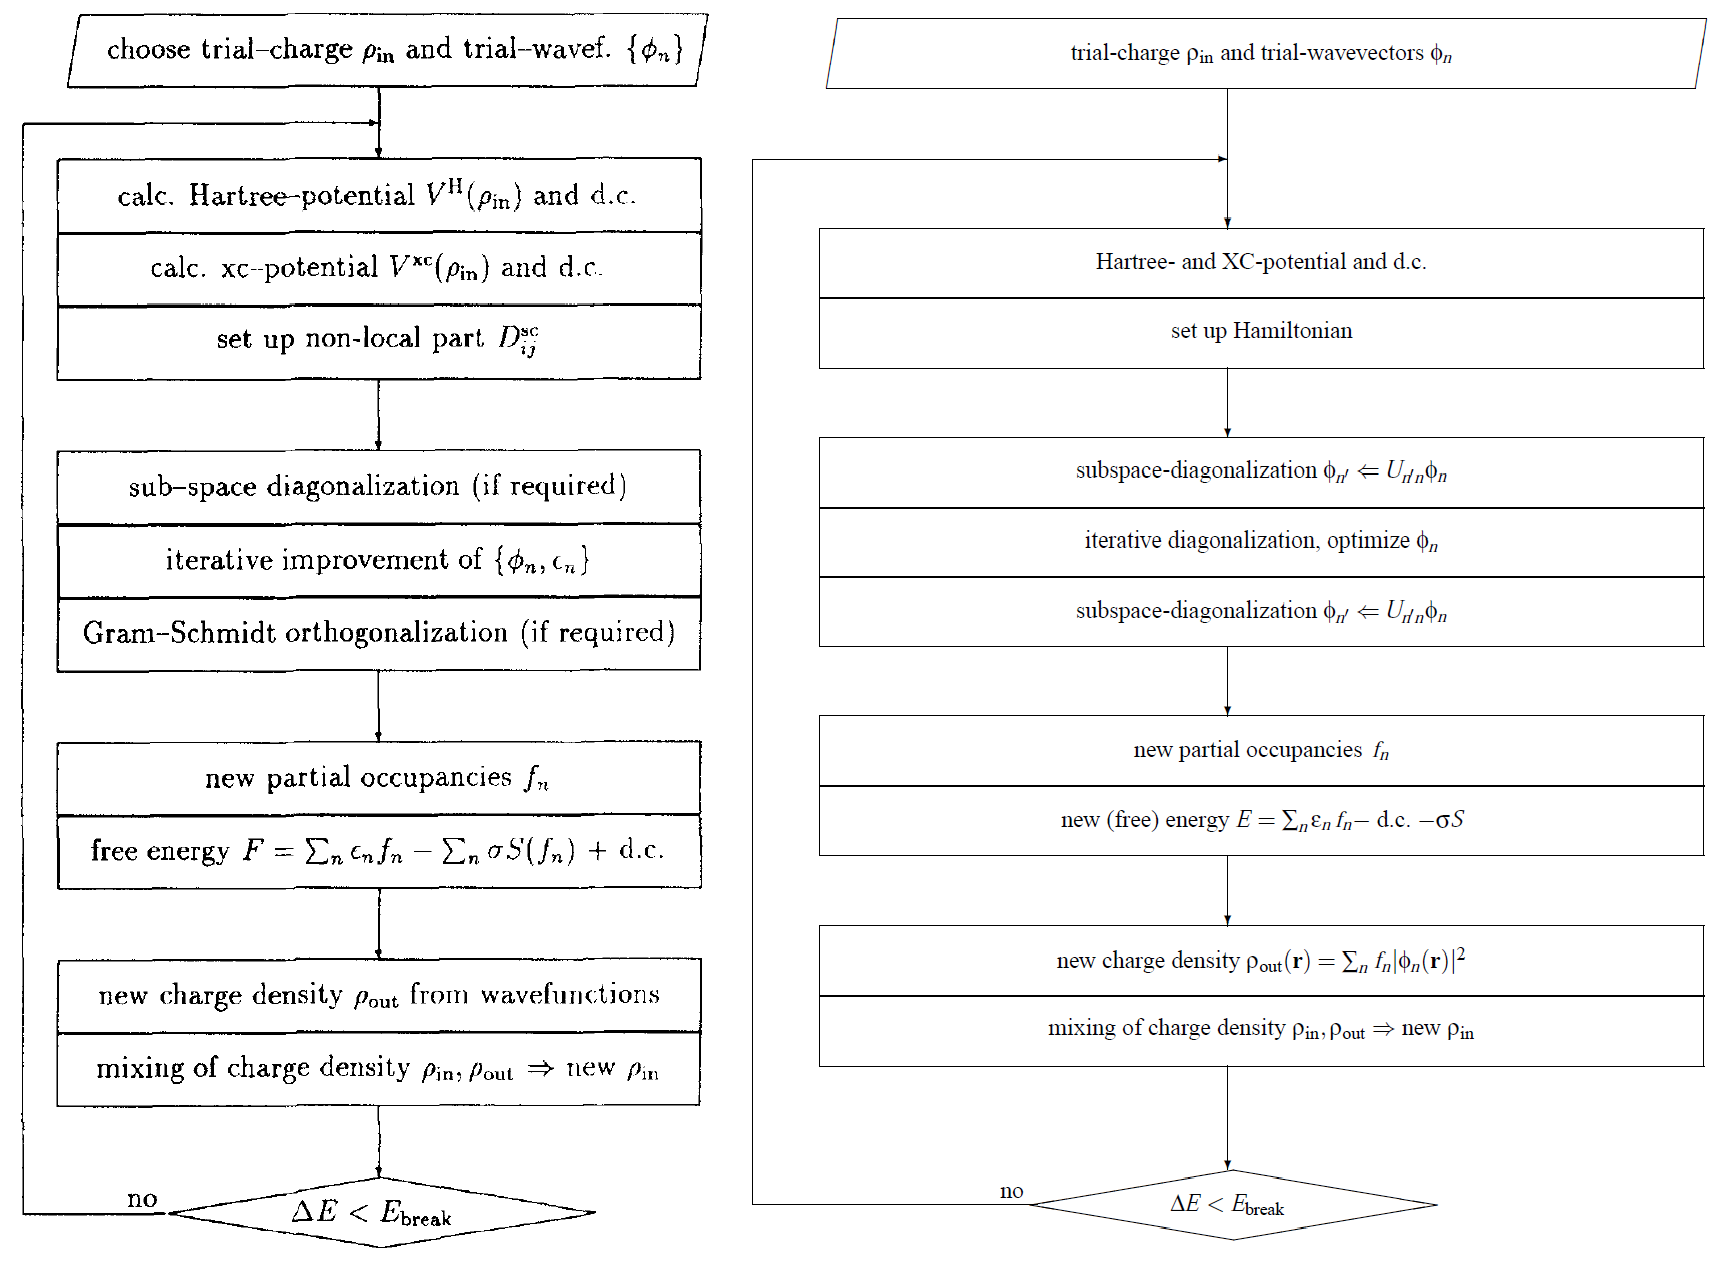
\includegraphics[height=2.7in,width=4.0in,viewport=0 0 1300 960,clip]{Figures/VASP_procedure-full.png}
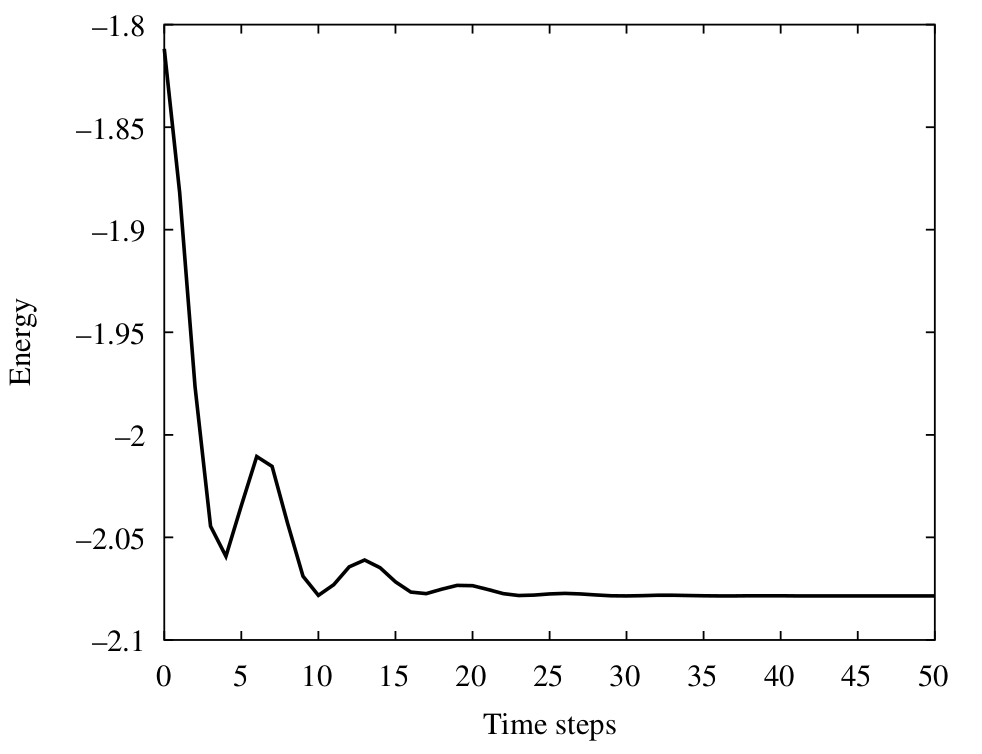
\includegraphics[height=1.5in,width=1.9in,viewport=0 0 740 600,clip]{Figures/Ab-initio-Ene.png}\\
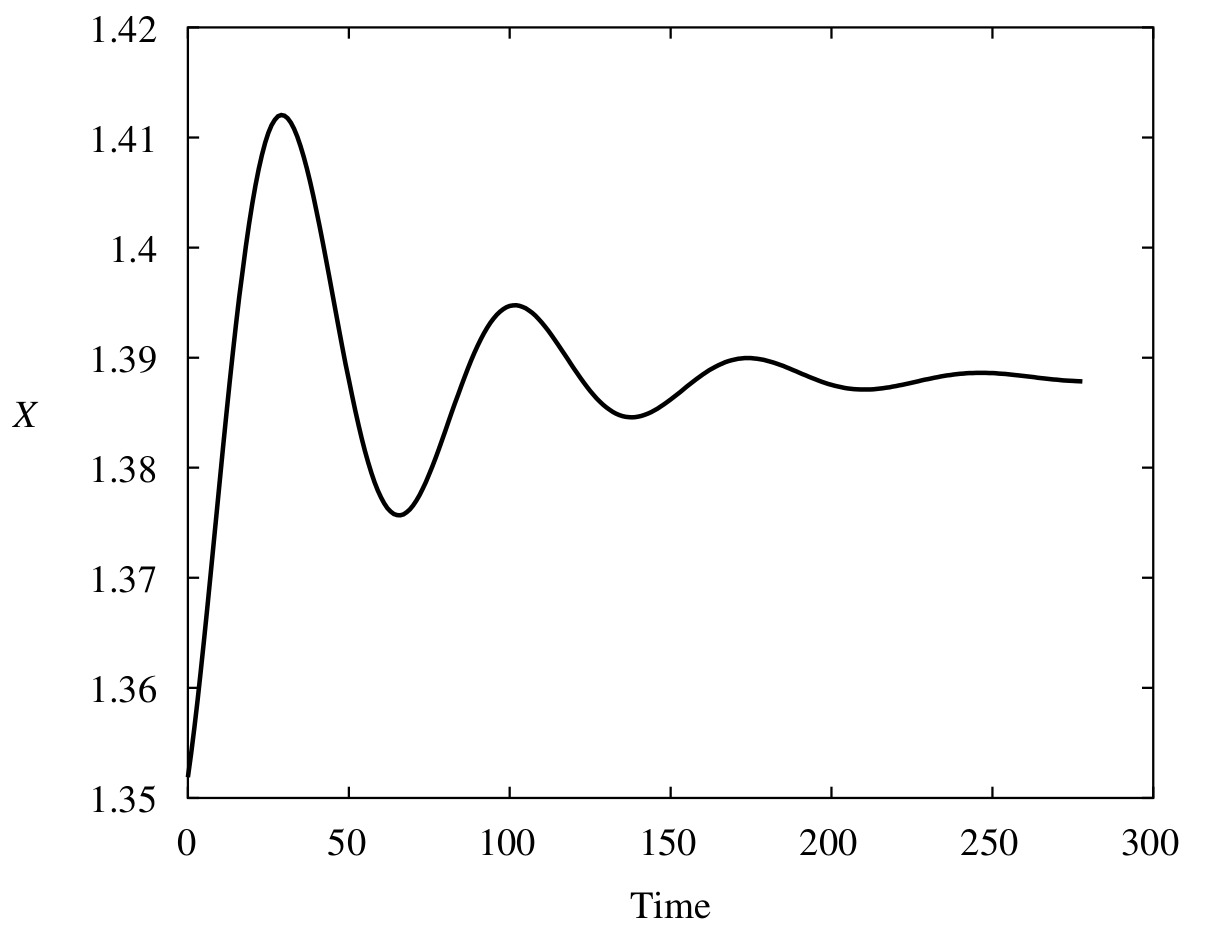
\includegraphics[height=1.5in,width=1.9in,viewport=0 0 1200 950,clip]{Figures/MD_H-R-rel.png}
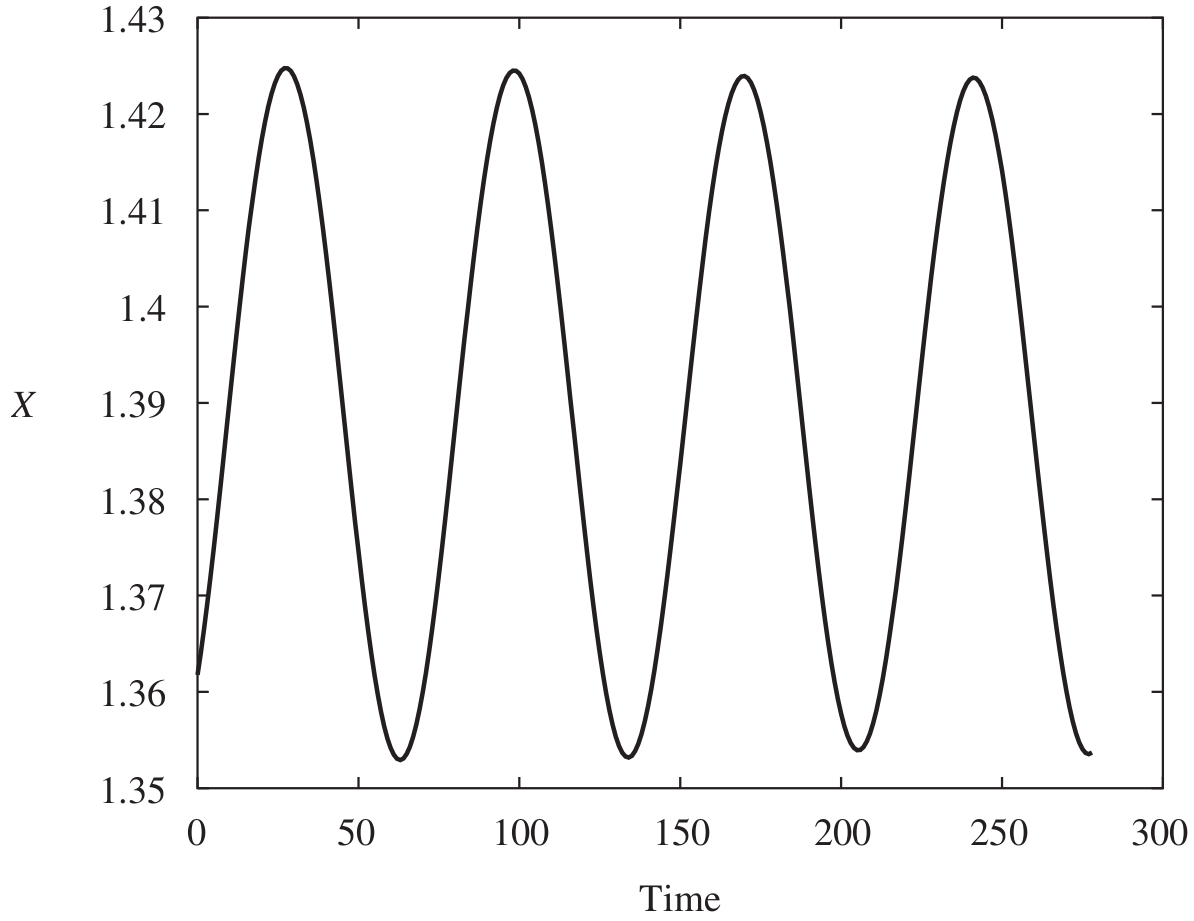
\includegraphics[height=1.5in,width=1.9in,viewport=0 0 1200 950,clip]{Figures/MD_H-R-MD.png}
\caption{\tiny \textrm{The Flow of calculation for the AIMD.}}%(与文献\cite{EPJB33-47_2003}图1对比)
\label{PAW_AIMD}
\end{figure} 
}


\frame
{
	\frametitle{波函数正交对计算的影响}
	{\fontsize{9.0pt}{5.2pt}\selectfont
	\textrm{Verlet}算法计算电子态波函数的运动方程
	\begin{displaymath}
		|\tilde\psi_k(t+h)\rangle=2|\psi_k(t)\rangle-|\psi_k(t-h)\rangle-\dfrac{2h^2}{\mu}(H|\psi_k(t)\rangle-\sum_l\Lambda_{kl}\psi_l)
	\end{displaymath}}
	当体系含有多个电子,\textrm{Langrage}乘子确保电子波函数彼此正交\\%,可有
	{\fontsize{7.0pt}{5.2pt}\selectfont
	实际上,存在多种正交方案
	\begin{itemize}
		\item 一次\textrm{unitary}变换产生一套正交轨道
			\begin{displaymath}
				\psi_k^{\prime}=\sum_lU_{kl}\psi_l
			\end{displaymath}
			这里基组$\{\psi_k^{\prime}\}$是正交的
		\item 一次波函数的\textrm{unitary}变化伴随\textrm{Lagtange}乘子的一次类似变换
			\begin{displaymath}
				\Lambda_{kl}^{\prime}=\sum_{mn}U_{km}^{\dagger}\Lambda_{mn}U_{nl}
			\end{displaymath}
	\end{itemize}
	不同的正交方案对应张开的空间相同,但张开空间的函数有所旋转
%	\begin{displaymath}
%		|\psi_k(t+h)\rangle=|\tilde\psi_k(t+h)\rangle+\sum_lX_{kl}|\psi_l(t)\rangle
%	\end{displaymath}
}\\
%	其中,{\fontsize{9.0pt}{5.2pt}\selectfont$X_{kl}=\dfrac{2h^2}{\mu}\Lambda_{kl}$},由此$|\psi_k(t+h)\rangle$正交\\
%	$X_{ij}$要求关于$\mathbf{X}$的矩阵方程
	{\fontsize{8.0pt}{5.2pt}\selectfont
	\textcolor{purple}{不同的旋转方式(不同的正交方案)会对\textrm{Verlet}算法的执行效率产生很大的影响}
%	\begin{displaymath}
%		\mathbf{X}\mathbf{X}^{\dag}+\mathbf{X}\mathbf{B}+\mathbf{B}^{\dag}\mathbf{X}^{\dag}=\mathbf{I}-\mathbf{A}
%	\end{displaymath}
}
%	能通过以下迭代快速收敛,这里{\fontsize{9.0pt}{5.2pt}\selectfont$A_{kl}=\langle\tilde\psi_k(t+h)|\tilde\psi_l(t+h)\rangle$},{\fontsize{9.0pt}{5.2pt}\selectfont$B_{kl}=\langle\psi_k(t)|\tilde\psi_l(t+h)\rangle$}
	{\fontsize{9.0pt}{5.2pt}\selectfont
%	\begin{displaymath}
%		\mathbf{X}^{(n+1)}=\frac12[\mathbf{I}-\mathbf{A}+\mathbf{X}^{(n)}(\mathbf{I}-\mathbf{B})+\mathbf{X}^{(n)}(\mathbf{I}-\mathbf{B}^{\dag})-\mathbf{X}^{n}\mathbf{X}^{(n){\dag}}]
%		\end{displaymath}
}
%	取初始{\fontsize{9.0pt}{5.2pt}\selectfont$\mathbf{X}=\frac12(\mathbf{I}-\mathbf{A})$}
}

%\subsection{电子态能量的最小化}
\frame[allowframebreaks]
{
	\frametitle{\textrm{Car-Parrinello}方法与平面波基}
	\begin{itemize}
		\item 推导总能对轨道自由度的受力
	{\fontsize{6.2pt}{5.2pt}\selectfont{
			\begin{displaymath}
				\begin{aligned}
					\dfrac{\partial E_{\mathrm{total}}}{\partial c_j^{\ast}(\vec K)}=&\dfrac{K^2}2c_j(\vec K)+\sum_{\vec K^{\prime}}V_{\mathrm{loc}}^{\ast}(\vec K-\vec K^{\prime})c_j(\vec K^{\prime})\\
					&+\sum_n\sum_{lm}F_{jlm}^n\mathrm{e}^{-\mathrm{i}\vec K\cdot\vec R_n}Y_{lm}(\hat{\vec K})h_{lm}^np_m^l(K)
				\end{aligned}
			\end{displaymath}
			这里$V_{\mathrm{loc}^{\mathrm{all}}}$是总局域势
			\begin{displaymath}
				V_{loc}(\vec K)=\sum_n\Delta V_{\mathrm{loc}}(\vec K)+V_{\mathrm{xc}}(\vec K)+4\pi\dfrac{n_{\mathrm{tot}}(\vec K)}{K^2}
			\end{displaymath}
		}}
		\item 推导总能对原子核的受力:\\
{\fontsize{6.2pt}{5.2pt}\selectfont{
			总能对原子位置坐标的梯度包括
			\begin{itemize}
{\fontsize{6.2pt}{5.2pt}\selectfont{
				\item 局域赝势部分的贡献
					\begin{displaymath}
						\nabla_{\vec R_n}E_{\mathrm{local}}=-\Omega\sum_{\vec K}\mathrm{i}\vec KV_{\mathrm{local,n}}(\vec K)\mathrm{e}^{-\mathrm{i}\vec K\cdot\vec R_n}n^{\ast}(\vec K)
					\end{displaymath}
				\item 非局域赝势部分的贡献
					\begin{displaymath}
						\nabla_{\vec R_n}E_{\mathrm{nonlocal}}=\sum_jf_j\sum_{l,m\varepsilon n}[(F_{jlm}^n)^{\ast}h_{lm}^n\nabla_{\vec R_n}F_{jlm}^n+\nabla_{\vec R_n}(F_{lm}^n)^{\ast}h_{lm}^nF_{lm}^n]
					\end{displaymath}
				\item 电子-核静电相互作用部分的贡献
					\begin{displaymath}
						\nabla_{\vec R_n}E_{\mathrm{ES}}=-\Omega\sum_{\vec K}\mathrm{i}\vec K\dfrac{n_{\mathrm{tot}}}{K^2}n_{\mathrm{core}}^n(\vec K)\mathrm{e}^{-\mathrm{i}\vec K\cdot\vec R_n}+\nabla_{\vec R_n}E_{\mathrm{ovrl}}
\end{displaymath}
				}}
			\end{itemize}
			其中
			\begin{displaymath}
				\nabla_{\vec R_n}F_{lm}^n=-\dfrac1{\sqrt{\Omega}}\sum_{\vec K}\mathrm{i}\vec K\mathrm{e}^{-\mathrm{i}\vec K\cdot\vec R_n}c_j^{\ast}(\vec K)Y_{lm}(\hat{\vec K})p_{lm}^l(\vec K)
			\end{displaymath}
			\begin{displaymath}
				\begin{aligned}
					\nabla_{\vec R_n}E_{\mathrm{ovrl}}=&\sideset{}{^{\prime}}\sum_{n^{\prime}}\sum_{\vec L}\bigg\{\dfrac{Z_nZ_{n^{\prime}}}{|\vec R_n-\vec R_{n^{\prime}}-\vec L|^3}\mathrm{erfc}\bigg[\dfrac{|\vec R_n-\vec R_{n^{\prime}}-\vec L|}{\sqrt{2(\xi_n^2+\xi_{n^{\prime}}^2)}}\bigg]\\
					&+\dfrac2{\sqrt{\pi}}\dfrac1{\sqrt{\xi_n^2+\xi_{n^{\prime}}^2}}\dfrac{Z_nZ_{n^{\prime}}}{|\vec R_n-\vec R_{n^{\prime}}-\vec L|^2}\mathrm{exp}\bigg[\dfrac{|\vec R_n-\vec R_{n^{\prime}}-\vec L|}{\sqrt{2(\xi_n^2+\xi_{n^{\prime}}^2)}}\bigg]\bigg\}\\
					&\times(\vec R_n-\vec R_{n^{\prime}}-\vec L)
				\end{aligned}
			\end{displaymath}
		}}
	\end{itemize}

}

\frame
{
	\frametitle{第一原理分子动力学提要}
	\textrm{Car-Parinello~}方法基本思想
	\begin{itemize}
		\item 只对原子核位置考虑受力$-\dfrac{\partial E_{\mathrm{tot}}}{\partial\vec R_n}$作用
		\item 电子结构是通过某种最小化方法确定能量泛函$E_{\mathrm{tot}}[\rho(\vec r)]$的极值得到,而非\textrm{Born-Oppenheimer}近似下的自洽迭代
		\item \textrm{Verlet}算法确定核位移过程中,并不要求在每一步核位移时,电子步充分弛豫到当前结构的基态
	\end{itemize}
	在\textrm{Car-Parinello}方法中,电子结构的计算变成经典的优化问题:~电子密度迭代过程中,约束条件下最小化问题
	\begin{itemize}
		\item 电子本征态波函数彼此正交约束下迭代对角化(内循环):\\
			\textcolor{blue}{子空间旋转}:~不同的正交化方法对迭代计算的影响
		\item 电荷密度混合过程中电荷数守恒约束(外循环)
			\begin{displaymath}
				\sum\limits_{j=0}^i a_j=1
			\end{displaymath}
	\end{itemize}
}

%------------------------------------------------------------------------Reference----------------------------------------------------------------------------------------------
		\frame[allowframebreaks]
{
\frametitle{主要参考文献}
\begin{thebibliography}{99}
{\tiny
	\bibitem{CMS6-15_1996}\textrm{G. Kresse and J. Furthm\"uller \textit{Comput. Mat. Sci.}, \textbf{6} (1996), 15}
	\bibitem{PRB54-11169_1996}\textrm{G. Kresse and J. Furthm\"uller \textit{Phys. Rev.} B, \textbf{54} (1996), 11169}
	\bibitem{PRL55-2471_1985}\textrm{R. Car and M. Parrinello \textit{Phys. Rev.} Lett., \textbf{55} (1985), 2471}
	\bibitem{PRB47-10142_1993}\textrm{K. Laasonen and A. Pasquarello and R. Car and C. Lee and D. Vanderbilt \textit{Phys. Rev.} B, \textbf{47} (1993), 10142}
	\bibitem{Chucizhangju}[东汉]王逸~撰. \textit{楚辞章句}\:上海古籍出版社, 上海, 2017
	\bibitem{Elect_Stru}\textrm{Richard. M. Martin. \textit{Electronic Structure: Basic Theory and Practical Methods} (Cambridge University Press, Cambridge, England, 2004)}
	\bibitem{Comp_Phys}\textrm{J. M. Thijssen. \textit{Computational Physics (2nd Edition)} (Cambridge University Press, Cambridge, England, 2007)}
        \bibitem{Singh}\textrm{D. J. Singh. \textit{Plane Wave, PseudoPotential and the LAPW method} (Kluwer Academic, Boston,USA, 1994)}					%
}
\end{thebibliography}
%\nocite*{}
}
%-----------------------------------------------------------------------------------------------------------------------------------------------------------------------%
\appendix
\subsection{经典数值优化算法概要}
\frame
{
	\frametitle{非线性方程的\rm{Newton~}法求根}
	\textcolor{blue}{不管哪一种数值算法,其设计原理都是将复杂转化为简单的重复,或者说,通过简单的重复生成复杂}:\\
	\textcolor{red}{在算法设计和算法实现过程中,重复就是力量}\\
迭代算法设计:~\textcolor{purple}{“速度”\textrm{vs}“稳定”}
\begin{figure}[h!]
\centering
\animategraphics[autoplay, loop, height=2.0in]{1}{Figures/OP_Newton_}{0}{17}
\label{Equation_Newon}
\end{figure}
}

\frame
{
	\frametitle{迭代优化基本思想}
	对于给定函数$f$,在极值点,函数的梯度满足
	\begin{displaymath}
		\nabla f=0
	\end{displaymath}
	可将函数极值问题转化成方程求根问题
\begin{figure}[h!]
\centering
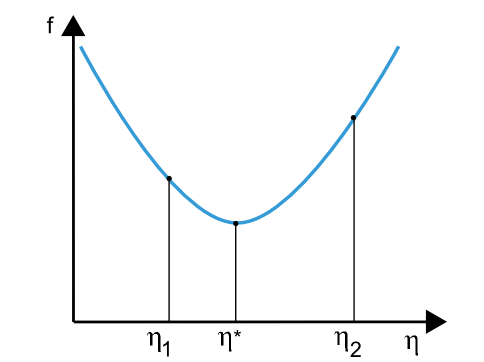
\includegraphics[height=1.68in,width=1.95in,viewport=30 0 450 360,clip]{Figures/OP_mini-1.png}
\hskip 0.05in
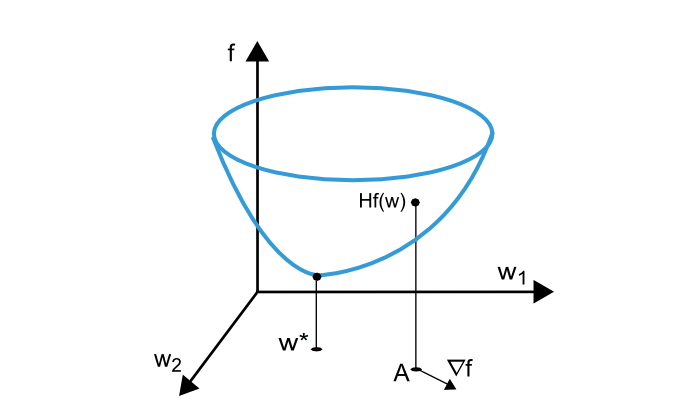
\includegraphics[height=1.68in,width=1.95in,viewport=150 20 560 390,clip]{Figures/OP_mini-2.png}
\label{OP_mini}
\end{figure}
}

\frame
{
	\frametitle{\textrm{Method of steepest descent}}
	对于函数$f(\mathbf{x}_0)$当前位置$\mathbf{x}_0$的负梯度方向$\mathbf{g}_0$满足
	\begin{displaymath}
		\mathbf{g}_0=-\nabla f(\mathbf{x}_0)
	\end{displaymath}
	用$\mathbf{g}_0$方向作为搜索方向,
	\begin{displaymath}
		\mathbf{x}=\mathbf{x}_0+\lambda\mathbf{g}_0,\qquad \lambda>0
	\end{displaymath}
	因为负的梯度方向为当前位置的最快下降方向,所以被称为“\textcolor{blue}{最陡下降法}”\\
	对函数$f$最小化参数$\lambda$,可确定下一步$\mathbf{x}_1$,可有
	\begin{displaymath}
		\dfrac{\mathrm{d}}{\mathrm{d}\lambda}f(\mathbf{x}_0+\lambda\mathbf{g})_0=\mathbf{g}_0\cdot\nabla f(\mathbf{x}_1)=\mathbf{g}_0\cdot\mathbf{g}_1=0
	\end{displaymath}
	因此\textcolor{red}{最速下降法最近邻两步的梯度彼此相互垂直}\\
	\textcolor{purple}{最陡下降法的收敛:~\\靠近极小值时收敛速度减慢,越接近目标,步长越小,前进越慢}
}

\frame
{
	\frametitle{\textrm{Newton-Raphson Method}}
	\textrm{Newton Method}是一种在实数和复数域上近似解方程的方法。\\
	思想:~\textcolor{blue}{用函数的\textrm{Taylor}级数的前几项来寻找方程$f(x)=0$的根}\\
	由\textrm{Newton}迭代公式有
	\begin{displaymath}
		x_{n+1}=x_n-\dfrac{f(x_n)}{f^{\prime}(x_n)}
	\end{displaymath}
	用\textrm{Taylor}级数在$a$附近展开$f(x)$
	\begin{displaymath}
		f(x)=\sum_{n=0}^{\infty}\dfrac{f^{(n)}(a)}{n!}(x-a)^n
	\end{displaymath}
	如果只取其前两项逼近$f(x)$,可有
	\begin{displaymath}
		f(x)=f(a)+f^{(1)}(a)(x-a)
	\end{displaymath}
	不难看出$x=a-\frac{f(a)}{f^{(1)}(a)}$时,有$f(x)=0$
}

\frame
{
	\frametitle{\textrm{Newton-Raphson Method}}
	对于函数求极值问题(函数的导数为零),就转换成
	\begin{displaymath}
		x_{n+1}=x_{n}-\dfrac{f^{(1)}(x_n)}{f^{(2)}(x_n)}
	\end{displaymath}
	对高维函数,一阶导数是梯度,二阶导数是\textcolor{blue}{\textrm{Hessian}矩阵}\\$\mathbf{H}f(\mathbf{x})=[\frac{\partial^2f}{\partial x_i\partial x_j}]_{n\times n}$,有
	\begin{displaymath}
		x_{n+1}=x_n-\alpha[\mathbf{H}f(x_n)]^{-1}\nabla f(x_n)\quad n\geqslant0
	\end{displaymath}
	这里$\alpha$是可调参数%,$\mathbf{H}$是\textrm{Hessian}矩阵

	\begin{itemize}
		\item 最陡下降法是用一个平面去拟合当前位置的局部曲面
		\item \textrm{Newton}法是用一个二次曲面拟合当前位置的局部曲面
	\end{itemize}
通常情况下,二次曲面的拟合会比平面更好,所以牛顿法选择的路径会更符合真实的最优下降路径(收敛更快)

\textcolor{magenta}{\textrm{Newton}法的缺点:~\textrm{Hessian}矩阵求逆的计算成本和复杂度较高}
}

\frame
{
	\frametitle{\textrm{Quasi-Newton Method}}
	\textrm{Newton}法收敛速度快,但计算过程中需计算\textrm{Hessian}矩阵(而且无法保证正定),因此有了\textrm{Quasi-Newton}方法\\
	思想:~\textcolor{blue}{构造可以近似\textrm{Hessian}矩阵(或逆)的正定对称阵}
		{\fontsize{7.2pt}{4.2pt}\selectfont{
	\begin{displaymath}
		f(\mathbf{x})\approx f(\mathbf{x}_{k+1})+\nabla f(\mathbf{x}_{k+1})(\mathbf{x}-\mathbf{x}_{k+1})+\dfrac12(\mathbf{x}-\mathbf{x}_{k+1})\nabla^2f(\mathbf{x}_{k+1})(\mathbf{x}-\mathbf{x}_{k+1})
	\end{displaymath}
	两边作用梯度算符$\nabla$
	\begin{displaymath}
		\nabla f(\mathbf{x})\approx\nabla f(\mathbf{x}_{k+1})+\mathbf{H}_{k+1}(\mathbf{x}-\mathbf{x}_{k+1})
	\end{displaymath}
	当$\mathbf{x}=\mathbf{x}_k$有
	\begin{displaymath}
		\mathbf{g}_{k+1}-\mathbf{g}_k\approx\mathbf{H}_{k+1}(\mathbf{x}-\mathbf{x}_k)
	\end{displaymath}
令
\begin{displaymath}
	\mathbf{s}_k=\mathbf{x}_{k+1}-\mathbf{x}_k\quad\mathbf{y}_k=\mathbf{g}_{k+1}-\mathbf{g}_k
\end{displaymath}
有
\begin{displaymath}
	\mathbf{y}_k\approx\mathbf{H}_{k+1}\cdot\mathbf{s}_k\quad\mbox{或}\quad\mathbf{s}_k\approx\mathbf{H}_{k+1}^{-1}\mathbf{y}_{k}
\end{displaymath}}}
{\fontsize{9.2pt}{4.2pt}\selectfont{\textcolor{purple}{\textrm{Quasi-Newton}法:~靠近极小值时收敛速快;~初值选择不好,易不收敛}}}
}

\frame
{
	\frametitle{共轭梯度的``轭''}
\begin{figure}[h!]
\centering
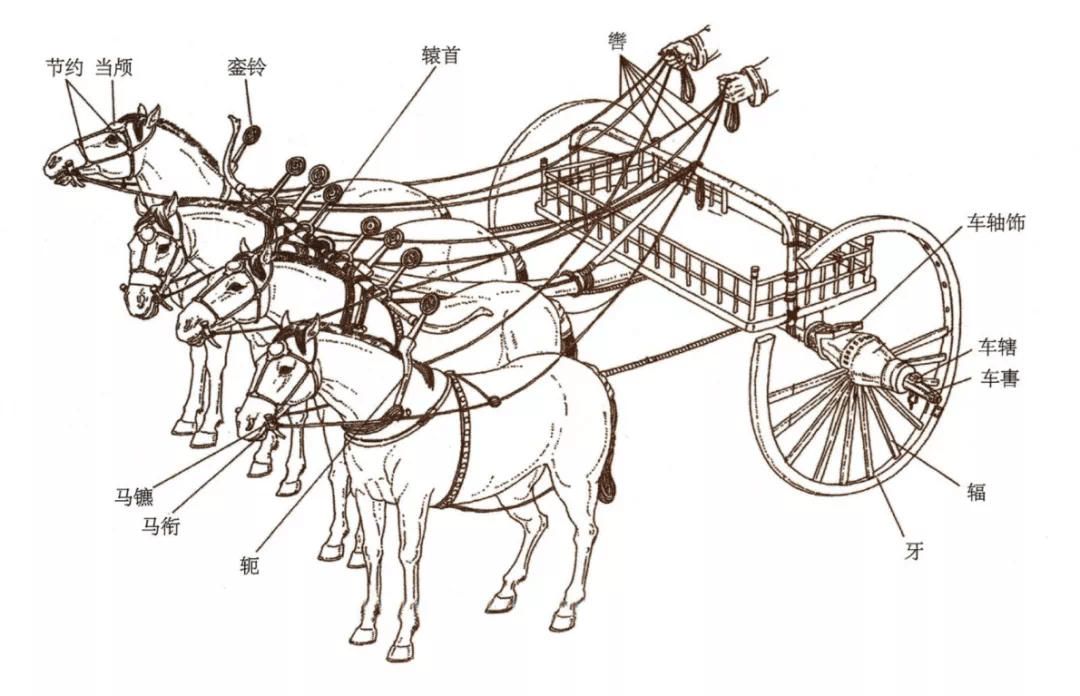
\includegraphics[height=2.5in,width=4.0in,viewport=0 0 1050 680,clip]{Figures/Yoke_1.png}
\label{Horse_Yoke}
%\caption{\tiny \textrm{Schematic illustration of minimization of a function in two dimensions. The steps 1,2,3,$\cdots$ denote the steepest descent steps and the point $2^{\ast}$ denote the conjugate gradient path that reaches the exact solution after two steps if the functional is quadratic.}}%(与文献\cite{EPJB33-47_2003}图1对比)
\end{figure}
}

\frame
{
	\frametitle{共轭的含义}
\begin{minipage}{0.63\textwidth}
\begin{figure}[h!]
\vskip -23pt
\centering
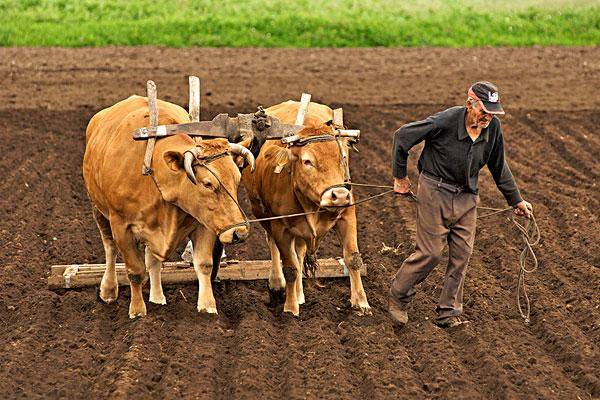
\includegraphics[height=1.6in,width=2.2in,viewport=0 0 600 490,clip]{Figures/Bi-Yoke_1.jpg}
\vskip 2pt
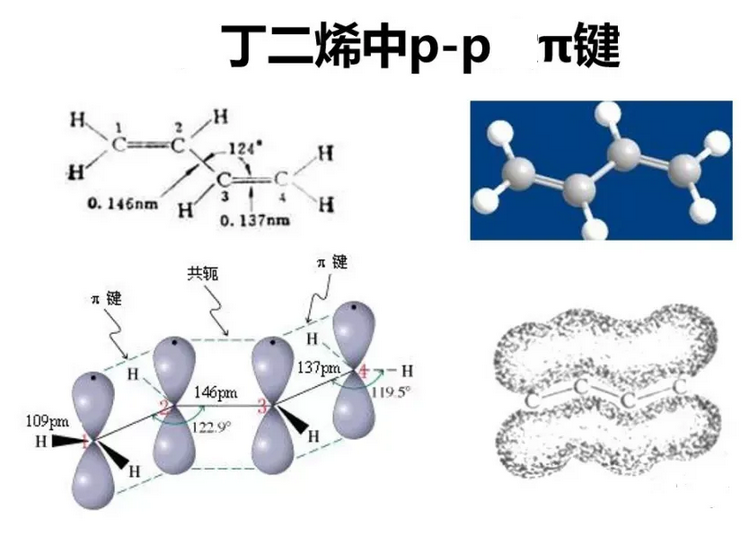
\includegraphics[height=1.5in,width=2.2in,viewport=0 0 750 530,clip]{Figures/Conjugate_Pi-bond.png}
\label{Conjugate_1}
%\caption{\tiny \textrm{Schematic illustration of minimization of a function in two dimensions. The steps 1,2,3,$\cdots$ denote the steepest descent steps and the point $2^{\ast}$ denote the conjugate gradient path that reaches the exact solution after two steps if the functional is quadratic.}}%(与文献\cite{EPJB33-47_2003}图1对比)
\end{figure}
\end{minipage}
\begin{minipage}{0.35\textwidth}
\begin{figure}[h!]
\centering
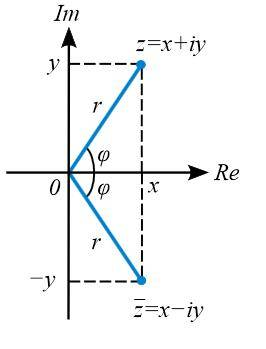
\includegraphics[height=2.2in,width=1.5in,viewport=0 0 250 390,clip]{Figures/Conjugate_complex.jpg}
\label{Conjugate_2}
%\caption{\tiny \textrm{Schematic illustration of minimization of a function in two dimensions. The steps 1,2,3,$\cdots$ denote the steepest descent steps and the point $2^{\ast}$ denote the conjugate gradient path that reaches the exact solution after two steps if the functional is quadratic.}}%(与文献\cite{EPJB33-47_2003}图1对比)
\end{figure}
\end{minipage}
}

\frame
{
	\frametitle{\textrm{Conjugate gradient}}
	假设函数在接近极值附件,近似有\textcolor{magenta}{二次函数}的形式
	\begin{displaymath}
		f(\mathbf{x})=f_0+\frac12\mathbf{x}\cdot\mathbf{H}{\mathbf{x}}+\cdots
	\end{displaymath}
	其中$\mathbf{H}$是\textcolor{blue}{\textrm{Hessian}矩阵}%,定义为
%	\begin{displaymath}
%		H_{ij}=\dfrac{\partial^2f(\mathbf{x})}{\partial x_i\partial x_j}
%	\end{displaymath}
	当$f$的偏导连续,则$\mathbf{H}$是对称矩阵,并且一般要求$\mathbf{H}$是正定的。相应的梯度表示为
	\begin{displaymath}
		\mathbf{g}=\nabla f(\mathbf{x})=-\dfrac{\partial f}{\partial\mathbf{x}}=-\mathbf{H}\cdot\mathbf{x}
	\end{displaymath}
	\vskip 20pt
	设从点$\mathbf{x}_i$出发沿方向$\mathbf{h}_i$(\textcolor{blue}{不再限于梯度$\mathbf{g}_i$方向}),前进到点$\mathbf{x}_{i+1}$,根据最小化要求
	\begin{displaymath}
		\mathbf{h}_i\cdot\nabla f(\mathbf{x}_{i+1})=0
	\end{displaymath}
	为确定$\mathbf{x_{i+1}}$点的继续前进方向$\mathbf{h}_{i+1}$,设$\mathbf{x}_{i+1}$可由$\mathbf{x}_i+\lambda\mathbf{h}_{i+1}$得到,因此$\mathbf{x}_{i+1}$的梯度
	\begin{displaymath}
		\mathbf{g}_{i+1}=\nabla f(\mathbf{x}_{i+1})=-\mathbf{H}\mathbf{x}_{i+1}=-\mathbf{H}(\mathbf{x}_{i}+\lambda\mathbf{h}_{i+1})
	\end{displaymath}
}

\frame
{
	\frametitle{\textrm{Conjugate gradient}}
	与方向$\mathbf{h}_i$相比,梯度的改变为
	\begin{displaymath}
		\Delta\mathbf{g}=-\lambda\mathbf{H}\mathbf{h}_{i+1}
	\end{displaymath}

	根据最小化要求,梯度的改变与$\mathbf{h}_i$方向正交
	\begin{displaymath}
		\mathbf{h}_i\cdot\mathbf{H}\cdot\mathbf{h}_{i+1}=0
	\end{displaymath}
	共轭梯度法算法:对于给定函数
	\begin{itemize}
		\item 已知初值$\mathbf{x}_0$和梯度$\mathbf{g}_0$,取初始方向$\mathbf{h_0}=\mathbf{g}_0$(\textcolor{blue}{最陡下降})
		\item 根据递推关系确定
			\begin{displaymath}
				\begin{aligned}
					\mathbf{g}_{i_+1}=&\mathbf{g}_{i_+1}-\lambda_i\mathbf{H}\mathbf{h}_{i}\qquad \lambda_i=\dfrac{\mathbf{g}_i\cdot\mathbf{g}_i}{\mathbf{g}_i\cdot\mathbf{H}\mathbf{h}_i}\\	
					\mathbf{h}_{i_+1}=&\mathbf{g}_{i_+1}+\gamma_i\mathbf{h}_{i}\qquad \gamma_i=-\dfrac{\mathbf{g}_{i+1}\cdot\mathbf{H}\mathbf{h}_i}{\mathbf{h}_i\cdot\mathbf{H}\mathbf{h}_i}\\	
					\mathbf{x}_{i_+1}=&\mathbf{x}_{i}+\lambda_i\mathbf{h}_{i}
				\end{aligned}
			\end{displaymath}
	\end{itemize}
	\textcolor{purple}{共轭梯度法的收敛:~步收敛性,稳定性高,不需要任何外来参数}
}

\frame
{
	\frametitle{最陡下降与共轭梯度}
\begin{figure}[h!]
\centering
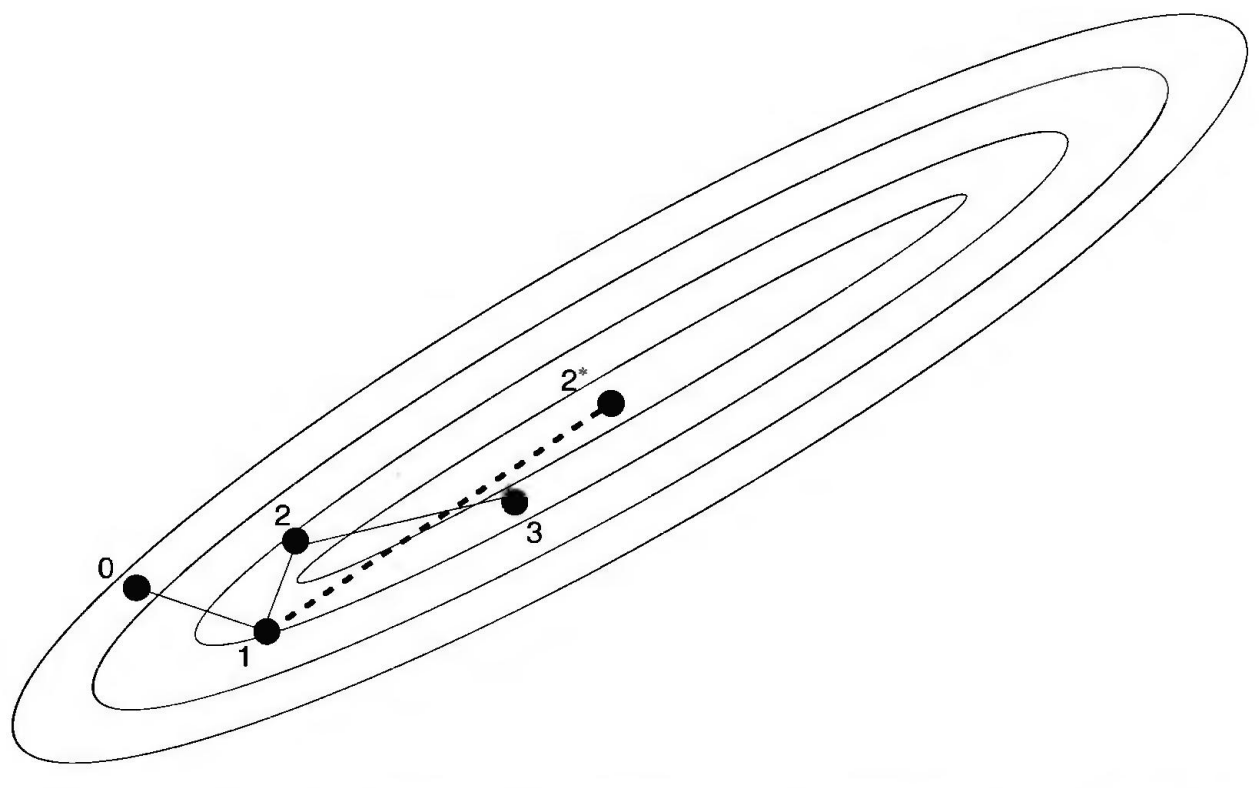
\includegraphics[height=2.0in,width=3.5in,viewport=0 0 950 590,clip]{Figures/OP_descent_CG.png}
\label{decent_CG}
\caption{\tiny \textrm{Schematic illustration of minimization of a function in two dimensions. The steps 1,2,3,~$\cdots$ denote the steepest descent steps and - \!- \!- \!- \!- \!- the point 2$^{\ast}$ denote the conjugate gradient path that reaches the exact solution after two steps if the functional is quadratic.}}%(与文献\cite{EPJB33-47_2003}图1对比)
\end{figure}
}

\frame
{
	\frametitle{不动点问题}
	求解方程
	\begin{displaymath}
		f(\mathbf{x})=\mathbf{x}
	\end{displaymath}
	$\mathbf{x}$是函数$f(\mathbf{x})$的\textcolor{red}{不动点}\textrm{Fixed Point}
	
	对这类问题的求解,可以利用迭代关系
	\begin{displaymath}
		\mathbf{x}_{i+1}=f(\mathbf{x}_i)\qquad (i=1,2,3,\cdots)
	\end{displaymath}
	这称为\textcolor{blue}{不动点迭代法}

	{\fontsize{6.2pt}{4.2pt}\selectfont{例如求解方程
	\begin{displaymath}
%		\begin{aligned}
			\lg(10+x)~=~x%\\
			\Longrightarrow	\textcolor{blue}{x\approx 1.04309063}
%		\end{aligned}
		\end{displaymath}}}
\begin{minipage}[b]{0.35\textwidth}
		{\fontsize{3.2pt}{1.2pt}\selectfont{
	\begin{displaymath}
	\vspace{-0.11in}
		\begin{aligned}
			x_0&=1 %~\Longrightarrow 
			\\\lg(10+1)&=1.041392685\\
x_1 &=1.041392685 %~\Longrightarrow 
\\\lg(10+1.041392685)&=1.0430238558\\
x_2 &=1.043023856 %~\Longrightarrow 
\\\lg(10+1.043023856)&=1.0430880104\\
x_3 &=1.043088010 %~\Longrightarrow 
\\\lg(10+1.043088010)&=1.0443090533\\
x_4 &=1.043090533 %~\Longrightarrow 
\\\lg(10+1.043090533)&=1.04430906326\\
x_4 &=1.0430906326 %~\Longrightarrow 
\\\lg(10+1.0430906326)&=1.04430906365\\
x_5 &=1.0430906365 %~\Longrightarrow 
\\\lg(10+1.0430906365)&=1.04430906366\\
x_6 &=1.0430906366 %~\Longrightarrow 
\\\lg(10+1.0430906366)&=1.04430906366
		\end{aligned}
	\end{displaymath}}}
\end{minipage}
\hfill
\begin{minipage}[b]{0.62\textwidth}
\begin{figure}[h!]
	\vspace{-0.21in}
\centering
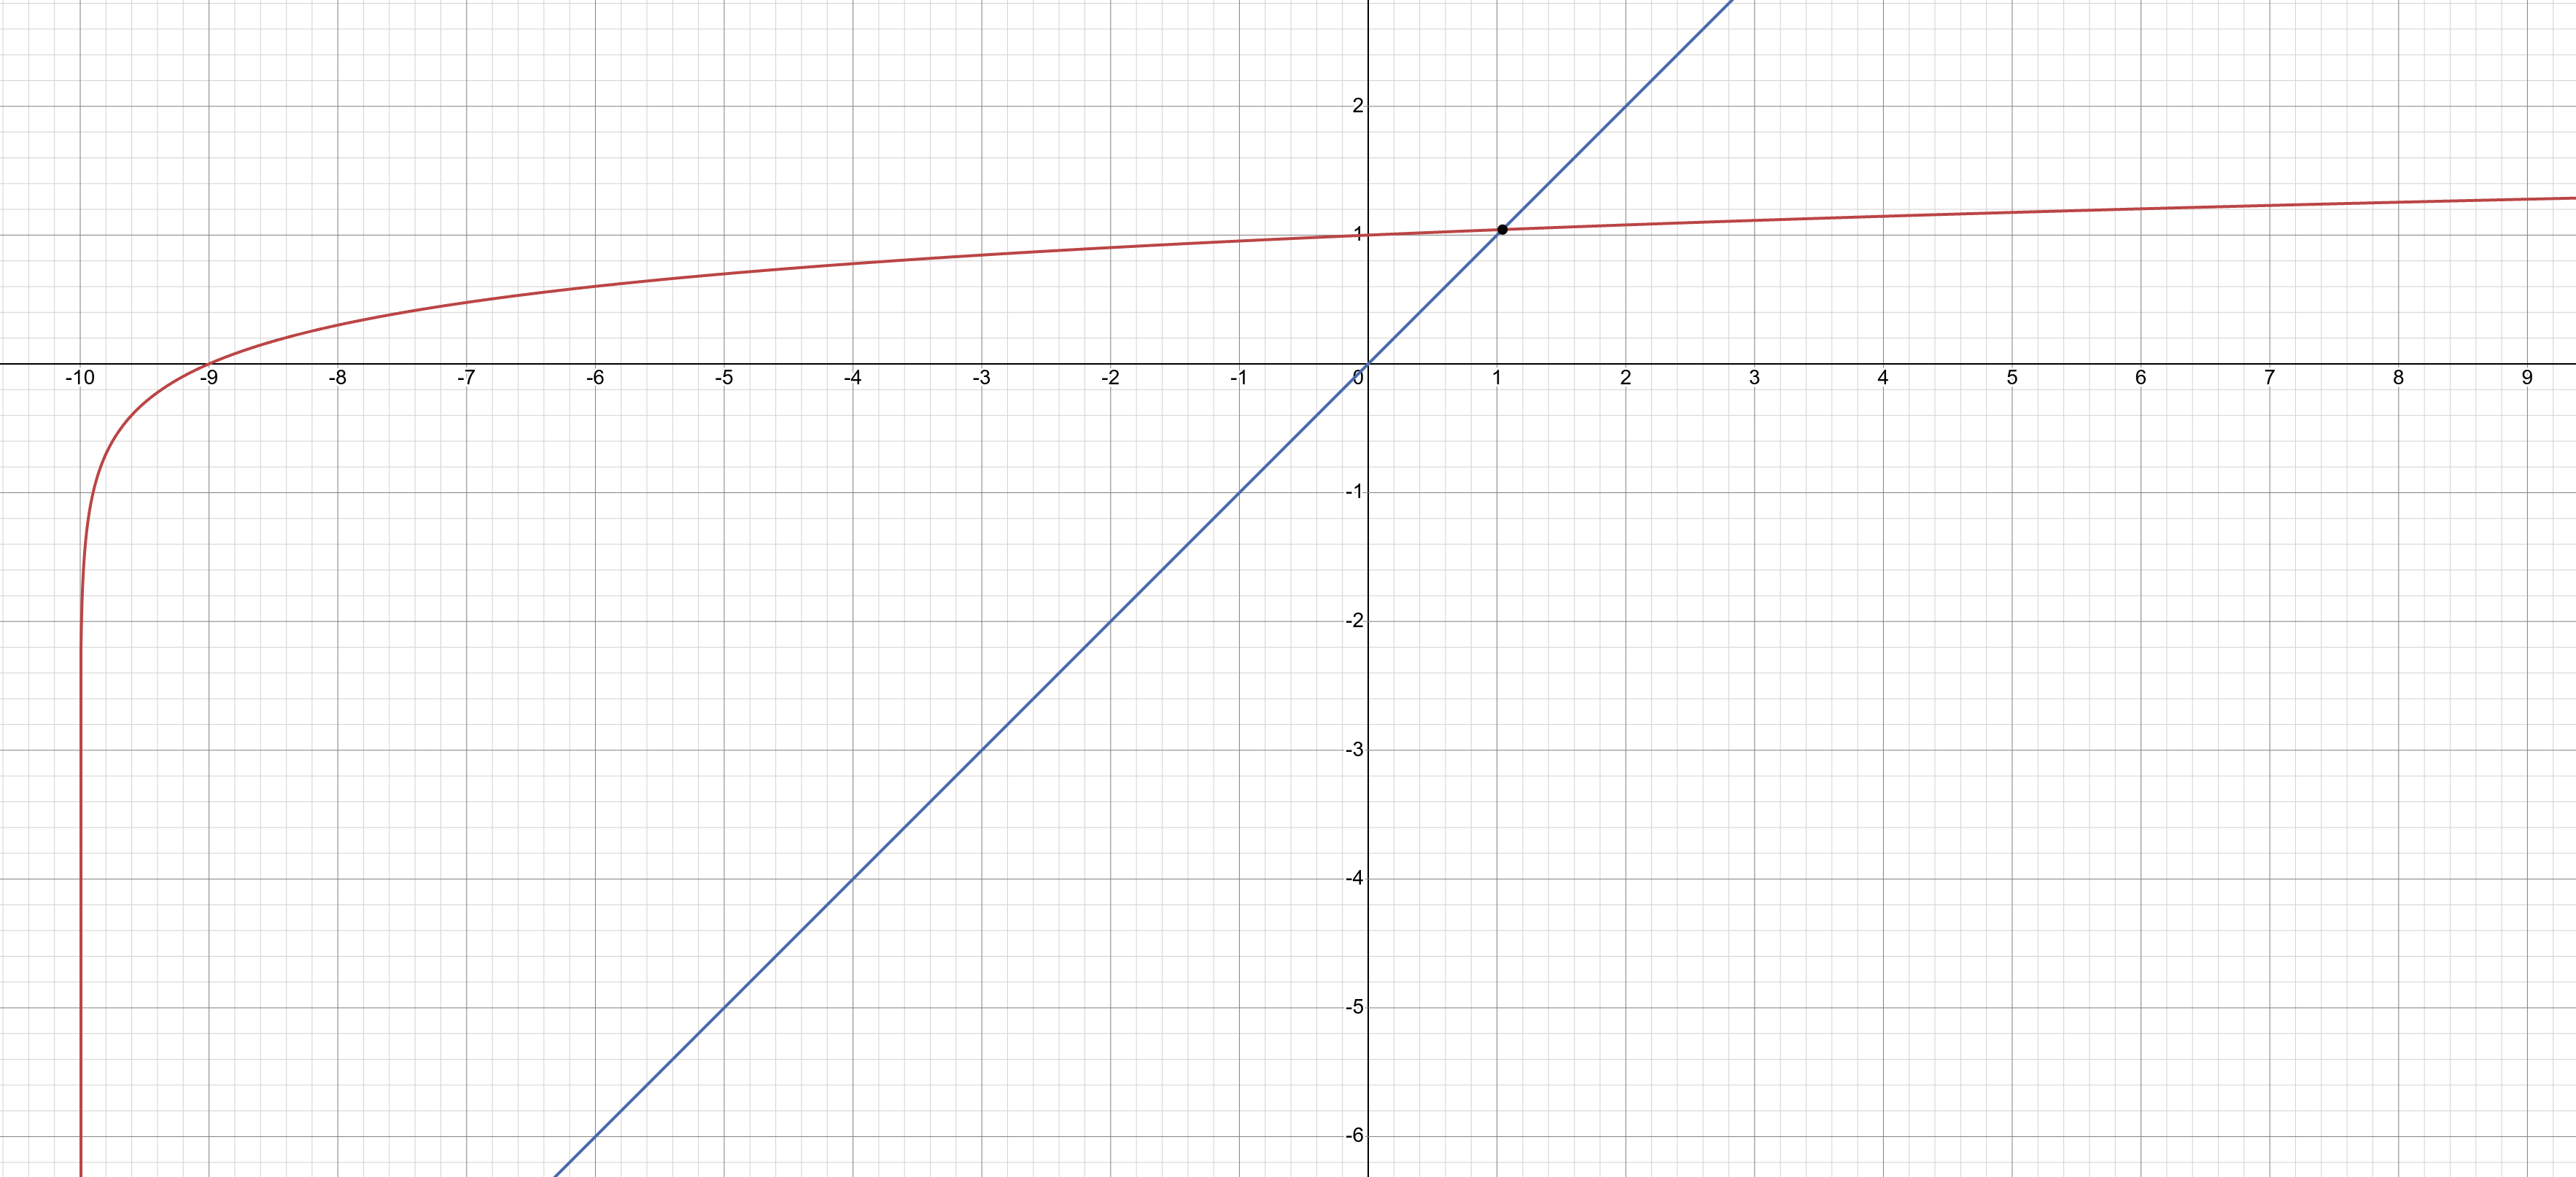
\includegraphics[height=1.3in,width=2.0in,viewport=0 0 2500 1600,clip]{Figures/solve_lg10.png}
%\caption{\tiny \textrm{The comparison of parallel scaling for ABINIT vs VASP.}}%(与文献\cite{EPJB33-47_2003}图1对比)
\label{solution-log_10}
\end{figure}
\end{minipage}
}

\frame
{
	\frametitle{\textrm{Residue minimization Methods}}
不动点迭代的主要问题是对初猜的依赖,很可能不收敛或线性收敛(收敛缓慢),一种求解策略是定义残量
	\begin{displaymath}
		R[\mathbf{x}]=f(\mathbf{x})-\mathbf{x}
	\end{displaymath}
	最小化残量的模$|R[\mathbf{x}]|$,特别是当残量$R[\mathbf{x}]$近似是$\mathbf{x}$的线性函数,可有\textcolor{purple}{\textrm{Jacobian}矩阵}
	\begin{displaymath}
		\mathbf{J}\equiv\dfrac{\delta R[\mathbf{x}]}{\delta\mathbf{x}}
	\end{displaymath}
	然后可以用\textrm{Quasi-Newton}方法最小化残量\\具体地可通过迭代关系求解原方程的解
	\begin{displaymath}
		\mathbf{x}_{i+1}=\mathbf{x}_{i}-\mathbf{J}^{-1}R[\mathbf{x}_{i}]
	\end{displaymath}
		但是一般来说\textrm{Jacobian}矩阵很可能未知(或者很难求逆),只有另图别策(在\textrm{Krylov}子空间中迭代求解),一般常用的方法有
		\begin{itemize}
			\item 迭代子空间求逆(\textrm{Discret Inversion in the Iterative Subspace,~DIIS})
			\item \textrm{Anderson}加速或\textrm{Anderson}混合
		\end{itemize}
}
	
\frame
{
	\frametitle{\textrm{Pulay DIIS full-subspace Metheod}}
	{\fontsize{7.2pt}{1.2pt}\selectfont{\textrm{DIIS}是\textrm{Pulay}引入的,俗称的\textcolor{blue}{\textrm{Pulay}混合}\footnote{\fontsize{5.2pt}{1.2pt}\selectfont{一般地说,\textrm{DIIS}是通用的不动点迭代的加速收敛方法;~对于线性问题,\textrm{DIIS}等价于\textrm{GMRES}方法}}}}\\
	{\fontsize{5.2pt}{1.2pt}\selectfont{其思想是:~对迭代逼近的矢量$\mathbf{x}_{i}$,可通过将之前得到的所有矢量$\mathbf{x}$线性组合得到,组合系数则由对其残矢最小化确定。概要如下\\
	在由$\mathbf{x}_i$构成的完全\textrm{Krylov}子空间内,有矢量
	\begin{displaymath}
		\mathbf{x}_{i+1}=\sum_{j=0}^{i}a_j\mathbf{x}_j=c_0\mathbf{x}_0+\sum_{j=1}^ic_j\delta\mathbf{x}_j
	\end{displaymath}
	若假设该矢量的残矢$R[\mathbf{x}_{i+1}]$与矢量$\mathbf{x}_{i+1}$满足相同的线性化要求
	\begin{displaymath}
		R[\mathbf{x}_{i+1}]=R[\sum_{j=0}^ia_j\mathbf{x}_j]=\sum_{j=0}^ia_jR[\mathbf{x}_j]
	\end{displaymath}
	通过最小化残矢的模
	\begin{displaymath}
		\langle R[\mathbf{x}_{i+1}]|R[\mathbf{x}_{i+1}]\rangle=\sum_{j,k}a_ja_kA_{j,k};A_{j,k}=\langle R[\mathbf{x}_j]|R[\mathbf{x}_k]\rangle
	\end{displaymath}
	即可确定矢量$\mathbf{x}_{i+1}$

	在电子结构计算中,残矢最小化的约束条件最常用的有
	\begin{itemize}
		\item 电子能带的本征矢正交
		\item 电荷密度混合时,电荷密度守恒,即$\sum\limits_{j=0}^i a_j=1$,可有\\\textcolor{blue}{$a_j=\sum\limits_jA_{j,i}^{-1}/\sum\limits_{j,k}a_ja_kA_{j,k}^{-1}=\sum\limits_jA_{j,i}^{-1}/\sum\limits_{j,k}A_{j,k}^{-1}$
%				\begin{displaymath}
%					\begin{aligned}
%						a_j=\sum\limits_jA_{j,i}^{-1}/\sum\limits_{j,k}&\underbrace{a_ja_k}A_{j,k}^{-1}\\
%						&\mbox{\textcolor{purple}{可略去}}
%					\end{aligned}
%				\end{displaymath}
		}
	\end{itemize}
}}
}

\frame
{
	\frametitle{\textrm{Broyden Jacobian update method}}
	最初的\textrm{Broyden}方法是\textcolor{magenta}{迭代过程中连续产生\textrm{Jacobian}逆阵的方案}
	{\fontsize{5.2pt}{1.2pt}\selectfont{
		\begin{itemize}
			\item 作为迭代起点,首先初猜合理的$\mathbf{J_0}^{-1}$(比如$\mathbf{J}_0^{-1}=\alpha\mathbf{I}$)
			\item 迭代开始的若干步内,保持$\mathbf{J}^{-1}$为初猜形式;~后续$\mathbf{J}^{-1}$再逐步更新:~
		因为$\mathbf{J}^{-1}$始终是近似的,有
				\begin{displaymath}
					\begin{aligned}
						\delta\mathbf{x}_i=&\mathbf{x}_i-\mathbf{x}_{i-1}=-\mathbf{J}_{i-1}^{-1}R_{i-1}\\
						\delta R_i=&R_i-R_{i-1}
					\end{aligned}
				\end{displaymath}
				因此要求每一步迭代更新的$\mathbf{J}_i^{-1}$满足
\begin{displaymath}
	0=\delta\mathbf{x}_i-\mathbf{J}_i^{-1}\delta R_i
\end{displaymath}
由此得到构成$M\times M$的$\mathbf{J}_i^{-1}$的$M$个方程
\item 最小化\textrm{Jacobian}逆阵的模变化
	\begin{displaymath}
		Q=||\mathbf{J}_{i}^{-1}-\mathbf{J}_{i}^{-1}||
	\end{displaymath}
	\textcolor{magenta}{\begin{displaymath}
			\mathbf{J}_i^{-1}=\mathbf{J}_{i-1}^{-1}\dfrac{(\delta\mathbf{x}_i-\mathbf{J}_i^{-1}\delta R_i)\delta R_i}{\langle\delta R_i|\delta R_i\rangle}
		\end{displaymath}}
		\end{itemize}
}}
	改进的\textrm{Broyden}方法与\textrm{DIIS}方法的结果类似,可以节约内存
	{\fontsize{5.2pt}{1.2pt}\selectfont{
	\begin{displaymath}
		Q^{\mathrm{modified}}=\sum_{j=1}^i w_j|\delta\mathbf{x}_j-\mathbf{J}_i^{-1}\delta R_j|^2+w_0||\mathbf{J}_i^{-1}-\mathbf{J}_0^{-1}||
	\end{displaymath}
	通过参数$w_j$筛选出迭代步中与之最密切关联的贡献
}}
}

\frame
{
	\frametitle{\textrm{Anderson acceleration}}
	\textrm{Donald~G.~Anderson}给出了加速不动点迭代的求解思路
	{\fontsize{7.2pt}{1.2pt}\selectfont{
	\begin{displaymath}
		\begin{aligned}
			\mathbf{x}_1=&f(\mathbf{x_0})\\
			\forall k=&1,2,\cdots\\
			&m_k=\min\{m,k\}\\
			&R_k=[R_{k-m_k},\cdots,R_k]\\
			&\alpha_k={\mathrm{argmin}}_{\alpha\in A_k}||R_k\alpha||_2,~\mbox{这里}A_k=\{\alpha=(\alpha_0,\alpha_1,\cdots,\alpha_{m_k})~\mbox{并满足}\sum\limits_{i=0}^n\alpha_i=1\}\\
			&\mathbf{x}_{k+1}=\sum_{i=0}^{m_k}(\alpha_k)_if_{k-m_k+i}
		\end{aligned}
	\end{displaymath}
}}
\begin{itemize}
	\item \textrm{Anderson}本质上是\textrm{Quasi-Newton}方法求解非线性方程(是割线方法的推广),也可以归入\textrm{Broyden}方法一类

	\item \textrm{Anderson}加速数学形式上可以看成\textrm{Generalized Minimal RESidual Method~(GMRES)}迭代推广到非线性方程求解,只是作了适当的截断
\end{itemize}
}

\frame
{
	\frametitle{\textrm{Anderson acceleration}}
	{\fontsize{6.2pt}{1.2pt}\selectfont{
	具体地,在迭代过程中,引入中间变量
	\begin{displaymath}
		\mathbf{x}_{i+1}^{\prime}=\alpha_k\mathbf{X}_k
	\end{displaymath}
	这里$\alpha_k$是组合系数$a_k\in A_k~$,~$\mathbf{X}_k=[\mathbf{x}_{k-m_k},\cdots, \mathbf{x}_k]$是含有最近$m_k+1$个矢量的矩阵\\
	选择合适的$\mathbf{x}_{k+1}^{\prime}$使得$||R(\mathbf{x}_{k+1}^{\prime})||$最小化

	因为$\alpha_k$的求和为1,有一阶近似
	\begin{displaymath}
		R(\mathbf{X}_k\alpha_k)=R\bigg(\sum_{i=0}^{m_k}(\alpha_k)_i\mathbf{x}_{k-m_k+i}\bigg)\approx\sum_{i=0}^{m_k}(\alpha_k)_iR(\mathbf{x}_{k-m_k+i})=R_k\alpha_k
	\end{displaymath}
	因此可以通过最小化$||R_k\alpha||_2$确定$\alpha$,进而确定$\mathbf{x}_{k+1}^{\prime}$
	
	考虑到$f(\mathbf{x})=\mathbf{x}$的精确解$\mathbf{x}^{\ast}$,因此$f(\mathbf{x}_{k+1}^{\prime})$可能比$\mathbf{x}_{k+1}^{\prime}$更接近$\mathbf{x}^{\ast}$,因此最终方程的解选为$\mathbf{x}_{k+1}=f(\mathbf{x}_{k+1}^{\prime})$而非$\mathbf{x}_{k+1}=\mathbf{x}_{k+1}^{\prime}$

类似地,因为$\alpha_k$的求和为1,有一阶近似
\begin{displaymath}
	f(\mathbf{x}_{k+1}^{\prime})=f\bigg(\sum_{i=0}^{m_k}(\alpha_k)_i\mathbf{x}_{k-m_k+i}\bigg)\approx\sum_{i=0}^{m_k}(\alpha_k)_if(\mathbf{x}_{k-m_k+i})=\sum_{i=0}^{m_k}(\alpha_k)_if_{k-m_k+i}
\end{displaymath}
最终确定方程的解为
\begin{displaymath}
	\mathbf{x}_{k+1}=\sum_{i=0}^{m_k}(\alpha_k)_if_{k-m_k+i}
\end{displaymath}
	}}
}

\subsection{矩阵的迭代对角化}
\frame
{
	\frametitle{矩阵的迭代对角化}
	\begin{itemize}
		\item 矩阵的直接对角化计算复杂复 $O(N^3)$
		\item 矩阵的迭代对角化计算复杂度 $O(N_0^2\times N\ln N)\quad N_0\ll N$
	\end{itemize}
	\textcolor{blue}{迭代求本征值的思想是\textrm{Jacobian~}于\textrm{1846~}年提出的}\upcite{Crelle30-51_1846}\\
	其基本思想是
	\begin{displaymath}
		(H-\varepsilon^n)|\psi^n\rangle=|R[\psi^n]\rangle
	\end{displaymath}
	这里$n$是迭代步数,$|\psi^n\rangle$和$\varepsilon^n$分别是本征态和本征值,$|R[\psi^n]\rangle$是残差矢量
	\vskip 10pt
	{\fontsize{7.2pt}{1.2pt}\selectfont{
	在电子态计算过程中,选择适当的基函数,可以使\textrm{Schr\"odinger~}方程的矩阵接近对角阵\\因此可有
	\begin{displaymath}
		\begin{aligned}
			|\psi^{n+1}\rangle=&\mathbf{D}^{-1}(\mathbf{H}-\varepsilon)|\psi^n\rangle+|\psi^n\rangle=\delta|\psi^{n+1}\rangle+|\psi^n\rangle\\
		\mathbf{D}\delta\psi^{n+1}=&R[\psi^n]
		\end{aligned}
	\end{displaymath}
	这里$\mathbf{D}$是非奇异矩阵,与$\mathbf{H}$矩阵有关,也叫''预处理矩阵'',可根据需要选取多种形式
	\begin{itemize}
		\item 要求$\mathbf{D}$比原始的$\mathbf{H}-\varepsilon$更易求逆阵
		\item 要求$\mathbf{D}$使得修正项$\delta\psi^{n+1}$能够使$\psi^n$尽可能接近正确的本征矢
	\end{itemize}
}}
}

\frame
{
	\frametitle{矩阵迭代对角化的基本思想}
\begin{figure}[h!]
\centering
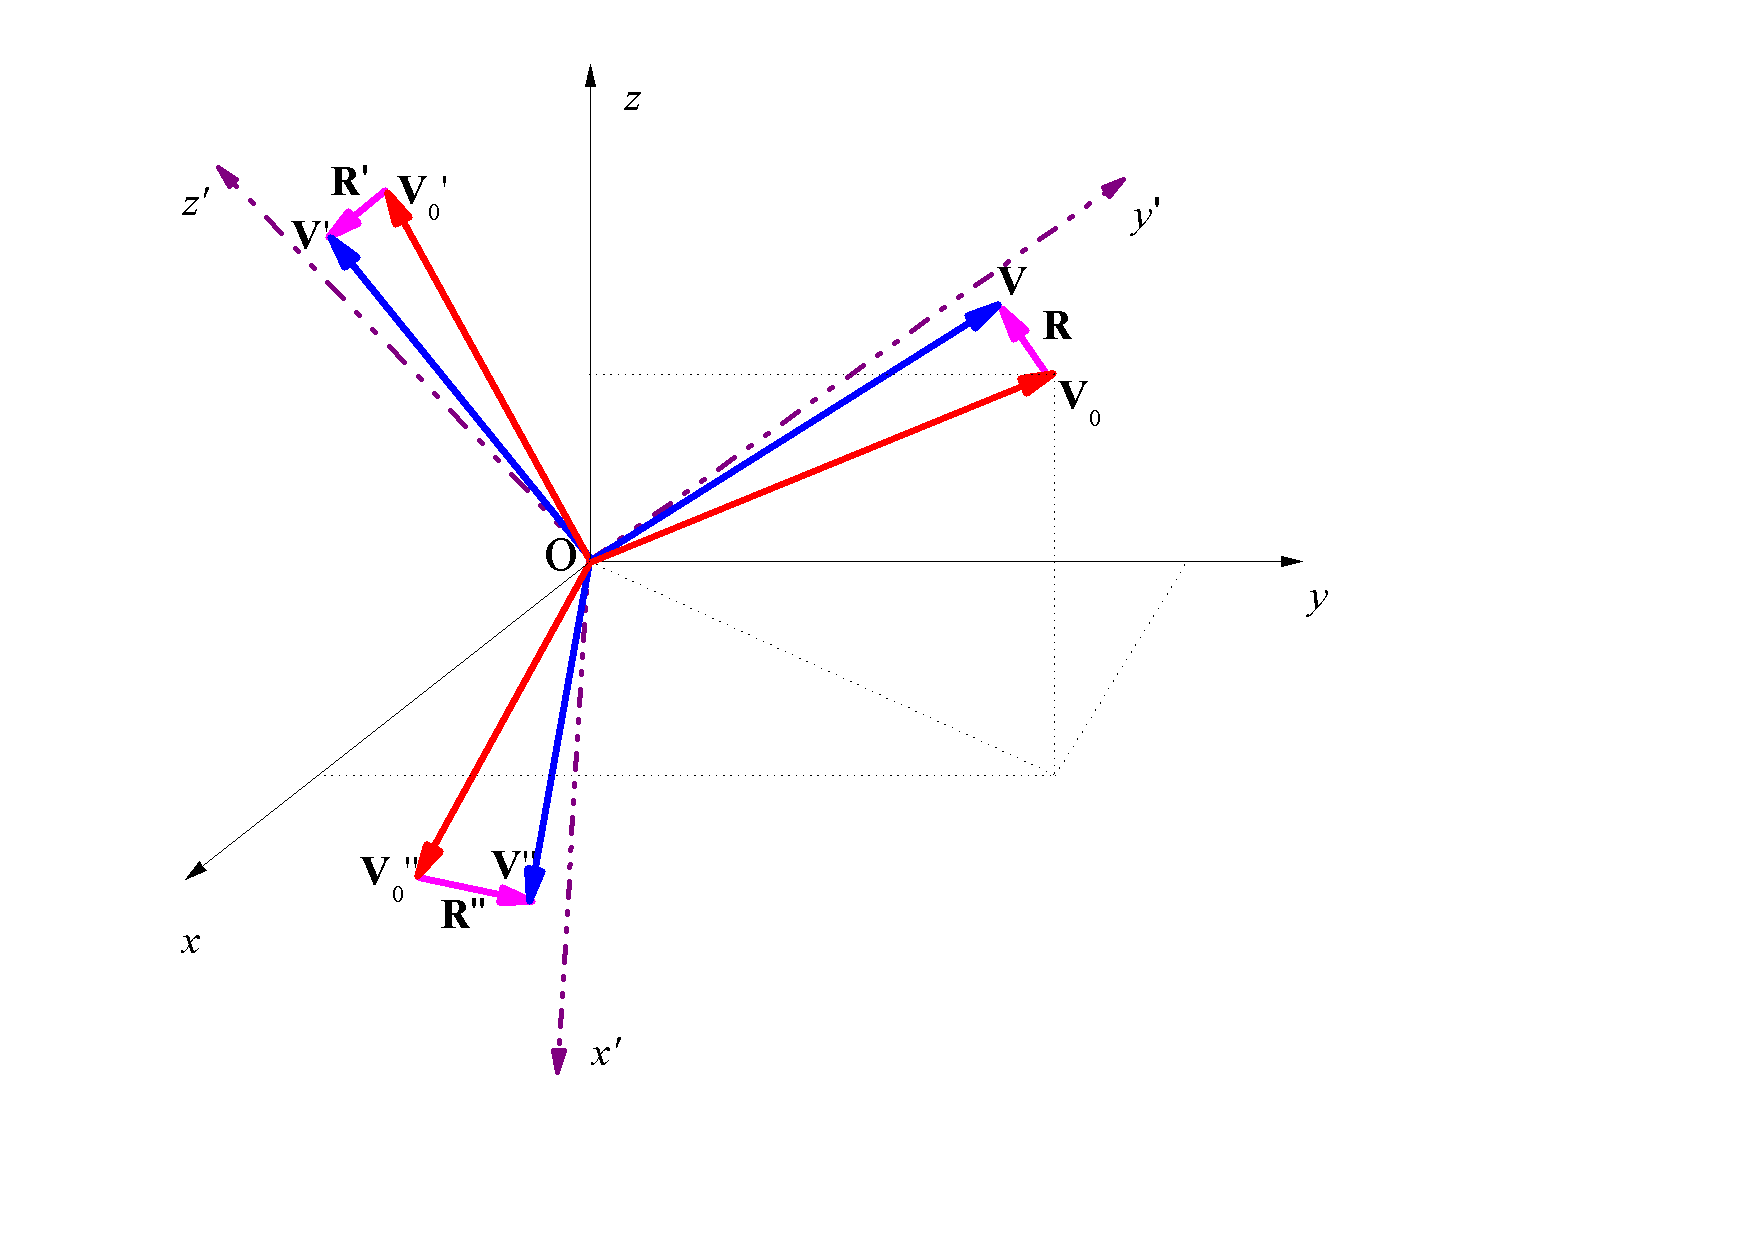
\includegraphics[height=2.5in,width=3.5in,viewport=0 0 850 590,clip]{Figures/Coordinate_transformation.png}
\label{decent_CG}
\caption{\tiny \textrm{Schematic illustration of searching for the eigenvalue of a vector.}}%(与文献\cite{EPJB33-47_2003}图1对比)
\end{figure}
}

\frame
{
	\frametitle{\textrm{Krylov}子空间与矩阵迭代}
	对于矩阵$\mathbf{A}$,取任意矢量$\psi_0$(要求归一),构造矢量$\psi_1$(同样要求归一,并与$\psi_0$正交),满足
	\begin{displaymath}
		\mathbf{A}\psi_0=a_0\psi_0+b_0\psi_1
	\end{displaymath}
	由此确定$a_0$、$b_0$、$\psi_1$
	\begin{displaymath}
		\begin{aligned}
			a_0&=\langle\psi_0|\mathbf{A}|\psi_0\rangle\\
			b_0\psi_1&=\mathbf{A}\psi_0-a_0\psi_0\\
			||\psi_1||&=1
		\end{aligned}
	\end{displaymath}
	进而可构造$\psi_2$:
	\begin{displaymath}
		\mathbf{A}\psi_1=c_1\psi_0+a_1\psi_1+b_1\psi_2
	\end{displaymath}
	要求$\psi_2$与$\psi_0$、$\psi_1$正交归一条件,确定$\psi_2$,$a_1$,$b_1$,$c_1$
}

\frame
{
	\frametitle{\textrm{Krylov}子空间与矩阵迭代}
	根据递推关系有
	\begin{displaymath}
		\mathbf{A}\psi_p=\sum_{q=0}^{p-1}c_p^{(q)}\psi_q+a_p\psi_p+b_p\psi_{p+1}
	\end{displaymath}
	这里$\psi_{p+1}$将与所有之前的$\psi_q$(\textrm{processors})正交

	利用矩阵$\mathrm{A}$的\textrm{Hermitian},因此对于$q<p-1$各项,可有等式
	\begin{displaymath}
		c_p^{(q)}=\langle\psi_q|\mathbf{A}\psi_p\rangle=\langle\mathbf{A}\psi_q|\psi_p\rangle=0
	\end{displaymath}
	即矢量$\psi_p$垂直于矢量$\mathbf{A}\psi_q$,由此可得
	\begin{displaymath}
		c_p^{(p-1)}=\langle\psi_{p-1}|\mathbf{A}\psi_p\rangle=\langle\mathbf{A}\psi_{p-1}|\psi_p\rangle=b_{p-1}
	\end{displaymath}
	经过$p$步迭代后
	\begin{displaymath}
		\mathbf{A}\psi_p=b_{p-1}\psi_{p-1}+a_p\psi_p+b_p\psi_{p+1}
	\end{displaymath}
	这里$\psi_{p+1}$要求与$\psi_p$和$\psi_{p-1}$满足正交归一条件
}

\frame
{
	\frametitle{矩阵对角化的\textrm{Lanczos~}算法}
	因此\textcolor{blue}{矩阵$\mathbf{A}$可以用$\psi_p$(称为\textrm{Lanczos}矢量)为基组表示成三对角阵形式}(稀疏矩阵)
	\begin{displaymath}
		\mathbf{A}^p=\begin{pmatrix}
			a_1 & b_2 & & & & \\
			b_2 & a_2 &b_3 & &\raisebox{0.8ex}[0pt]{\huge{0}} &\\
&b_3 &a_3 &\ddots & & \\
& &\ddots &\ddots &b_{p-1} & \\
& & &b_{p-1} &a_{p-1} &b_{p}\\
&\raisebox{0.8ex}[0pt]{\huge{0}} & & &b_{p} &a_{p}
		\end{pmatrix}
	\end{displaymath}
	不难看出,\textcolor{blue}{经过$p$次\textrm{Lanczos}迭代,当$b\rightarrow0$即达到收敛,意味着此时$p\times p$三对角阵$\mathbf{A}^p$的本征值也将收敛到矩阵$\mathbf{A}$的本征值}
	\begin{itemize}
		\item 稀疏矩阵$\mathbf{A}^p$可通过快速\textrm{QR}分解得到本征值
		\item 三对角阵的最低和最高本征值随着迭代次数增加收敛最迅速
		\item \textrm{Lanczos}方法适用于少量本征值与剩余本征有较大差值的体系
	\end{itemize}
}

\frame
{
	\frametitle{矩阵对角化的\textrm{Lanczos~}算法}
	大型稀疏矩阵对角化基本思路便是从一个试探向量$\mathbf{c}_0$出发,通过矩阵-向量乘操作\footnote{\fontsize{5.2pt}{1.2pt}\selectfont{由于矩阵是稀疏的,从而可以快速进行矩阵-向量乘这一基本操作(时间复杂度$\mathrm{O}(N^2)$)}},同时保持矩阵的稀疏性,使得试探向量逐渐收敛到目标特征向量(往往是基态对应的特征向量)

	{\fontsize{6.2pt}{1.2pt}\selectfont{
		本征值求解对应如下优化问题
		\begin{displaymath}
			\lambda_{\min}=\mathrm{min}_{\mathbf{c}}\rho(\mathbf{c})=\mathrm{min}_{\mathbf{c}}\dfrac{\mathbf{c}^\mathbf{H}\mathbf{c}}{\mathbf{c}^T\mathbf{c}}
		\end{displaymath}
		利用最陡下降法求解上述优化问题,则需要计算函数的梯度
		\begin{displaymath}
			\nabla\rho(\mathbf{c})|_{\mathbf{c}=\mathbf{c}_0}=\dfrac2{\mathbf{c}^T\mathbf{c}}(\mathbf{H}\mathbf{c}_0-\rho(\mathbf{c}_0)\mathbf{c}_0)
		\end{displaymath}
		实际计算中无需求出梯度并作精确搜索,因为\textcolor{blue}{解一定在\textrm{Krylov}子空间$\mathrm{span}(\mathbf{c}_0,\mathbf{H}\mathbf{c}_0)$内;~只需计算这两个向量之间的哈密顿矩阵元,并对角化所得到的小矩阵便相当于做了一步最速下降法}

		经过$k$步迭代之后所得到的解在子空间$\mathrm{span}(\mathbf{c}_0,\mathbf{H}\mathbf{c}_0,\cdots),\mathbf{H}^k\mathbf{c_0}$

		因此\textcolor{magenta}{大型矩阵对角化的问题,转化为子空间内矩阵对角化的问题}

		选取合适的初猜,经过若干次迭代之后,子空间内最小特征值可能于真实的最小特征值非常接近\footnote{\fontsize{5.2pt}{1.2pt}\selectfont{子空间内若干个最小特征值都可能于相应的真值非常接近}}

		一般地,$k$次迭代后第$j$个特征向量写成
		\begin{displaymath}
			\mathbf{c}_j^{(k)}=\sum_{i=0}^kc_{i,j}^{(k)}\mathbf{H}^i\mathbf{c}_0
		\end{displaymath}
	}}
}

\frame
{
	\frametitle{矩阵迭代对角化}
	稀疏矩阵求解的\textrm{Lanczos}优化过程,只变动一个分量$\mathbf{c}_I$的前提下
	\begin{displaymath}
		\dfrac{\partial\rho}{\partial\mathbf{c}_I}\bigg|_{\mathbf{c}_I+\delta_I}=0
	\end{displaymath}
	是可以精确求解的,其解为
	\begin{displaymath}
		\delta_I=(\rho(\mathbf{c}_0)-\mathbf{H}_{II})^{-1}\mathbf{q}_I\qquad\mbox{这里}\mathbf{q}=(\mathbf{H}-\rho\mathbf{I})\mathbf{c}_0
	\end{displaymath}
	不难看出,矢量$\mathbf{q}$就对应\textrm{Jacobi}迭代中用于判断收敛的残差矢量

更一般地,求解方程
	\begin{displaymath}
		\dfrac{\partial\rho}{\partial\mathbf{c}}\bigg|_{\mathbf{c}+\mathbf{\delta}}=0
	\end{displaymath}
	将方程展开到二阶近似,不难有
	\begin{displaymath}
		(\rho-\mathbf{H}_{II})\delta_I\approx \mathbf{q}_I+\sum_{J\neq I}\delta_J+(\rho-\lambda)\mathbf{c}_I
	\end{displaymath}
	实际计算中选则$\delta_I=(\rho(\mathbf{c}_0)-\mathbf{H}_{II})^{-1}\mathbf{q}_I$并不是方程的解的好的近似,\textcolor{purple}{好处是计算比较简单}
}

\frame
{
	\frametitle{\textrm{Block-Davison algorithm}}
	\textrm{Davidson}方法是求解大型稀疏矩阵的少量本征值问题提出来的,结合了\textrm{Lanczos}优化和\textrm{Jacobi}迭代的优点,简言之就是改进初猜,不用$\mathbf{H}\mathbf{c}_0$,而改用计算简单的$\delta_I=(\rho(\mathbf{c}_0)-\mathbf{H}_{II})^{-1}\mathbf{q}_I$形式
	\vskip 10pt
	应用\textrm{Davison}方法可以快速地依次求解稀疏矩阵的少量本征值和本征矢,将该方法推广为同时求解若干个本征态,即块-\textrm{Davidson}方法
	{\fontsize{6.2pt}{1.2pt}\selectfont{
		\begin{itemize}
			\item 选取合适数目正交归一的向量$\mathbf{c}_1,\mathbf{c}_2,\cdots, \mathbf{c}_n$作为初猜子空间的基组, 计算并储存向量$\mathbf{H}\mathbf{c}_i$和矩阵元$\mathbf{H}=\langle\mathbf{c}_i|\mathbf{H}|\mathbf{c}_j\rangle$ 
			\item 对角化矩阵,得到本征值$\lambda^{n}$和本征矢$\mathbf{a}^{n}$
			\item 构造残量矢量$\mathbf{q}_M=(\mathbf{H}-\lambda^{(M)}\mathbf{I})\mathbf{a}^{(M)}~\mbox{其中}\mathbf{a}^{(M)}=\sum\limits_{i=1}^M a_i^{(M)}\mathbf{a}_i$
			\item 根据模长$||\mathbf{q}_M||$判断迭代收敛情况
			\item 构造$\delta_{I,M+1}=(\lambda^{(M)}-\mathbf{H}_{II})^{-1}\mathbf{q}_{I,M}$,与此前的基组正交归一化,得到$\mathbf{c}_{M+1}$
			\item 计算矩阵元$\mathbf{H}_{i,M+1}\quad i=1,2,\cdots, M+1$
			\item 对角化矩阵得到新的本征值和本征矢量,继续迭代
		\end{itemize}
	}}
}

\frame
{
	\frametitle{\textrm{RMM-DIIS}}
	{\fontsize{7.2pt}{1.2pt}\selectfont{前述矩阵迭代对角化方法的优化策略都是
	\begin{itemize}
		\item 通过迭代优化得到最小本征值(极值)
		\item 利用本征态正交,依次获得其他各本征态和本征值
	\end{itemize}}}
	{\fontsize{7.2pt}{1.2pt}\selectfont{\textrm{RMM-DIIS~(Residual Minimization Method by Direct Inversion in the Iterative Subspace)}\footnote{\fontsize{5.2pt}{1.2pt}\selectfont{\textrm{RMM-DIIS}的得名源自该方法的提出者\textrm{Pulay}:~该方法的基本思想是在历次迭代产生的矢量构成的完整\textrm{Krylov}子空间内,完成对残矢的最小化}}方法则可以不用引入正交条件而得到多个本征值,\textcolor{purple}{因为该方法最小化的不是本征值而是残矢}}}\\
	{\fontsize{5.2pt}{1.2pt}\selectfont{
		其基本思想概要:~在$n$维\textrm{Krylov}子空间内,生成矢量
		\begin{displaymath}
			\psi^{n+1}=c_0\psi^0+\sum_{j=1}^{n+1}c_j\delta\psi^{j}
		\end{displaymath}
		通过改变选取一套合适的系数$c_j$来完成$\psi^{n+1}$的残矢$R^{n=1}$的最小化。\textcolor{blue}{等价于$c_j$由$\{\psi^0,\psi^1,\cdots,\psi^n\}$构成的\textrm{Krylov}子空间内求\textrm{Hermitian}本征值问题}
		\begin{displaymath}
			\sum_{j=1}^n\langle R^i|R^j\rangle c_j=\varepsilon\sum_{j=1}^n\langle\psi^i|\mathbf{S}|\psi^j\rangle c_j
		\end{displaymath}
		每迭代一次,子空间引入一个新波函数$\psi$和一个新残矢$R(\psi)$
		\begin{itemize}
			\item \textrm{RMM-DIIS}的计算量瓶颈将是后续的逐个矩阵-向量乘操作$\textrm{H}\psi$
%				\\因此要避免直接用\textrm{RMM-DIIS}直接处理大规模本征态~(但可以是大体系中的少量本征态)
			\item 只要内存许可,\textrm{RMM-DIIS}构造的完整的子空间内,构成子空间的矢量本征值都可以求解出来
			\item 因为\textrm{RMM}方法对初猜的矢量敏感(矢量收敛的位置到离初猜较近)
		\end{itemize}
%		\textrm{RMM-DIIS}最大的优点是一次可以得到多个本征态和本征值,而且不需要正交化
	}}
}

%-----------------------------------------------------------------------------------------------------------------------------------------------------------------------%
		\frame[allowframebreaks]
{
\frametitle{主要参考文献}
\begin{thebibliography}{99}
{\tiny
	\bibitem{Crelle30-51_1846}\textrm{C. G. Jacobi,\textbf{\"Uber ein leichtes Verfahren die in der Theorie der S\"acul\"arst\"orrungen vorkommenden Gleichungen numerisch aufzul\"osen}, \textit{Crelle's J.} \textbf{30} (1846), 51-94}
	\bibitem{Elect_Stru}\textrm{Richard. M. Martin. \textit{Electronic Structure: Basic Theory and Practical Methods} (Cambridge University Press, Cambridge, England, 2004)}
	\bibitem{Comp_Phys}\textrm{J. M. Thijssen. \textit{Computational Physics (2nd Edition)} (Cambridge University Press, Cambridge, England, 2007)}
}
\end{thebibliography}
%\nocite*{}
}
%-----------------------------------------------------------------------------------------------------------------------------------------------------------------------%
